\documentclass[11pt]{article}
\usepackage{epsf}
\usepackage{hyperref}
\usepackage{graphicx}
\usepackage{subfigure}
\usepackage[margin=2.5cm]{geometry}
\usepackage{amsmath}
\usepackage{footnote}
\usepackage[bottom]{footmisc}
\usepackage[singlelinecheck=false]{caption}
\usepackage{caption}
\usepackage{amsthm}
\usepackage{enumitem}
\usepackage{graphics}
\usepackage{float}
\usepackage{amssymb}
\usepackage{natbib}
\usepackage{lscape}
\usepackage{array}
\textheight=8.7in
\usepackage{setspace}
\usepackage{verbatim}
\usepackage{multirow}

\def\threedigits#1{%
  \ifnum#1<100 0\fi
  \ifnum#1<10 0\fi
  \number#1}

\topmargin=0.1in \oddsidemargin=-0.1cm \evensidemargin=-0.1cm

\paperheight=11in \paperwidth=8.5in \marginparwidth=0in

\marginparsep=0in \textwidth=6.5in \headheight=0in \headsep=0in

\onehalfspacing
\def\argmax{\mathop{\rm arg\,max}}
%\usepackage{xspace,epsfig,subfig}
\newtheorem{theorem}{Theorem}
\newtheorem{lemma}{Lemma}
\newtheorem{claim}{Claim}
\newtheorem{proposition}{Proposition}
\newtheorem{definition}{Definition}
\newtheorem{corollary}{Corollary}
\newenvironment{sketch}{\noindent\emph{Proof Sketch:}}{$\quad \Box$}
%\newenvironment{proof}{\noindent\emph{Proof:}}{$\quad \Box$}

\bibpunct{(}{)}{;}{a}{,}{,}

\newcommand{\E}{\operatorname{E}}

\begin{document}
\title{Estimating the number of clusters using Cross Validation}
\author{Wei Fu \qquad Patrick O. Perry \\\\ New York University}
\date{}
\maketitle
\begin{abstract}
Many clustering methods, including K-means, require the user to specify the number of clusters as an input parameter. A variety of methods have been devised to choose the number of clusters automatically, but they often rely on strong modeling assumptions. We propose a data-driven approach to estimate the number of clusters based on a novel form of cross-validation. This differs from ordinary cross-validation, because clustering is fundamentally an unsupervised learning problem. Simulation and real data analysis results show that our proposed method outperforms existing methods, especially in high-dimensional settings with heavy-tailed data.
\end{abstract}

\section{Introduction}
As a main task of exploratory data analysis, clustering organizes unlabeled observations into groups such that observations in same group are more similar compare to those in different group. Clustering is an important topic in unsupervised learning because it can reveal the internal structure of data through grouping, segment the data through partitioning and summarize data for other purposes such as dimension reduction. It has being widely used in various fields such as psychology, biology, statistics and machine learning including pattern recognition, image segmentation etc.\\

After being proposed more than $50$ years, $K$-mean remains one of the most popular and widely used clustering algorithms \citep{jain2010data}. Like many other clustering methods, $K$-mean requires an input parameter $k$, the number of clusters, to be specified by the user. Automatically and quantitatively deciding such parameter is important and yet unsolved problem \citep{fujita2014non}. Various methods have been proposed to tackle this difficulty. One ad hoc approach is to explore the relationship between $W_k$ (within-cluster dispersion) and the number of cluster $k$ for a certain clustering method such as $K$-mean. Since $W_k$ decreases as $k$ increases, one usually find the ``elbow" of curve $W_k$ \textsl{VS} $k$ as the appropriate number of clusters. The example on the top row of Figure \ref{fig1} demonstrates such approach for data with $k=4$, where the ``elbow" point indeed reveals the true number of clusters. This is based on the idea that under partitioning data set has more impact than over partitioning data set in terms of $W_k$. However, locating the ``elbow" point is somewhat subjective and sometimes is not appropriate to select the optimal $k$. The second example on the bottom row of Figure \ref{fig1} shows a  situation where there is no clear choice of the ``elbow" point -- both $k=2$ and $k=3$ can be viewed as the ``elbow" point. What's more, the true $k=4$ can never be selected as the optimal $k$ using such approach in this case since it can hardly be viewed as the ``elbow" of the curve.
\begin{figure}
\begin{minipage}{\linewidth}
\centering
\begin{minipage}{0.45\linewidth}
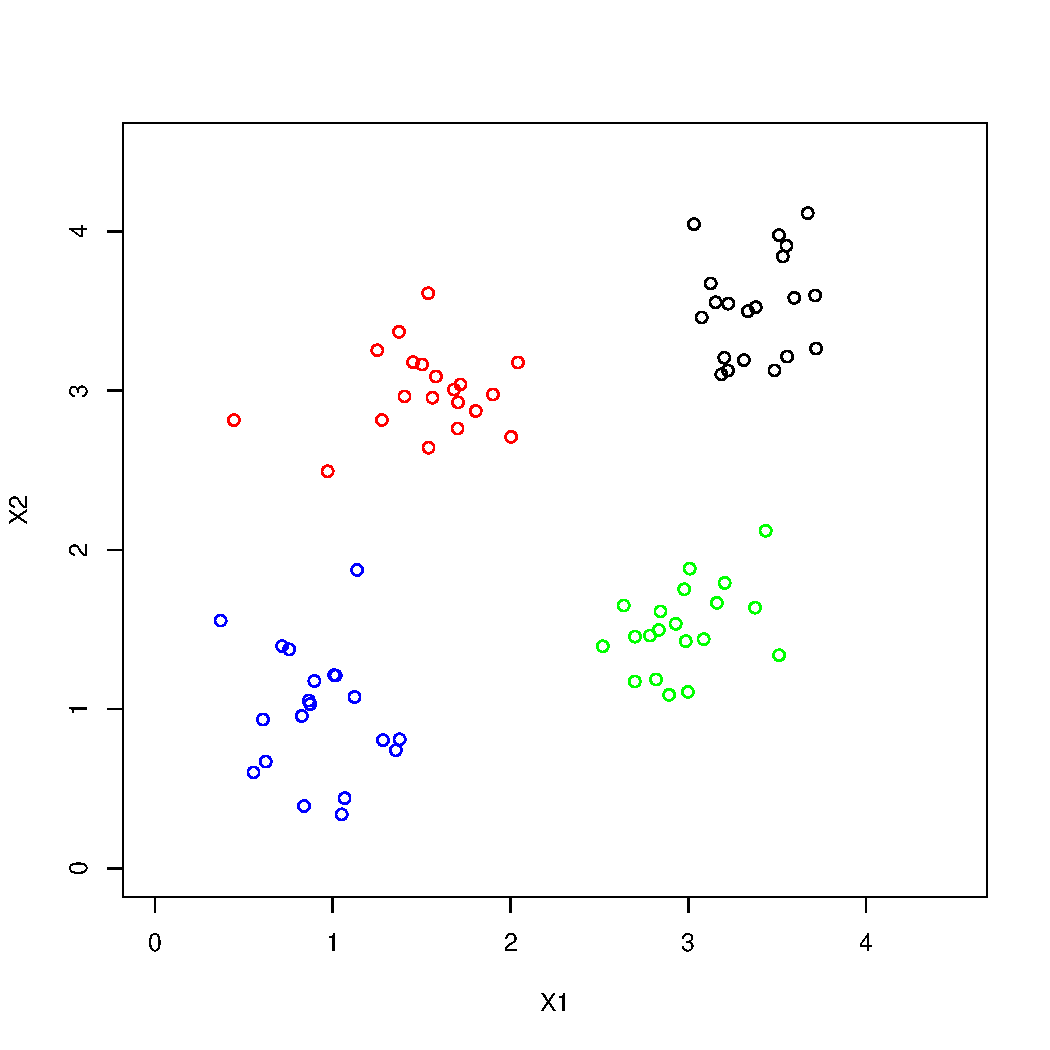
\includegraphics[width=\linewidth]{figure/Data_example.pdf}
\end{minipage}
\hspace{0.05in}
\begin{minipage}{0.45\linewidth}
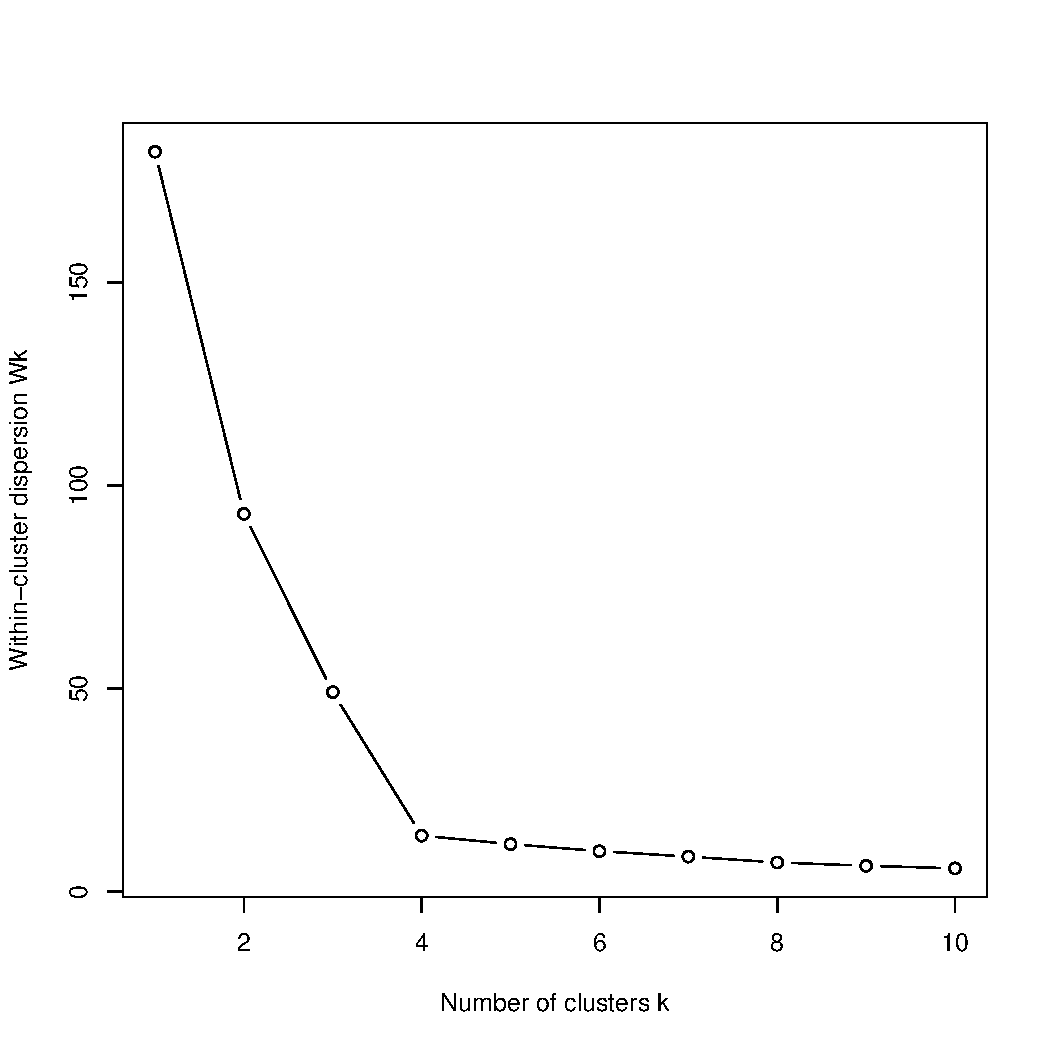
\includegraphics[width=\linewidth]{figure/W_k.pdf}
\end{minipage}
\end{minipage}
%\center{\caption{\label{fig1} Left plot shows the actual data, and the right plot shows the $W_k$ \textsl{VS} $k$ curve. }}
%\end{figure}

%\begin{figure}
\begin{minipage}{\linewidth}
\centering
\begin{minipage}{0.45\linewidth}
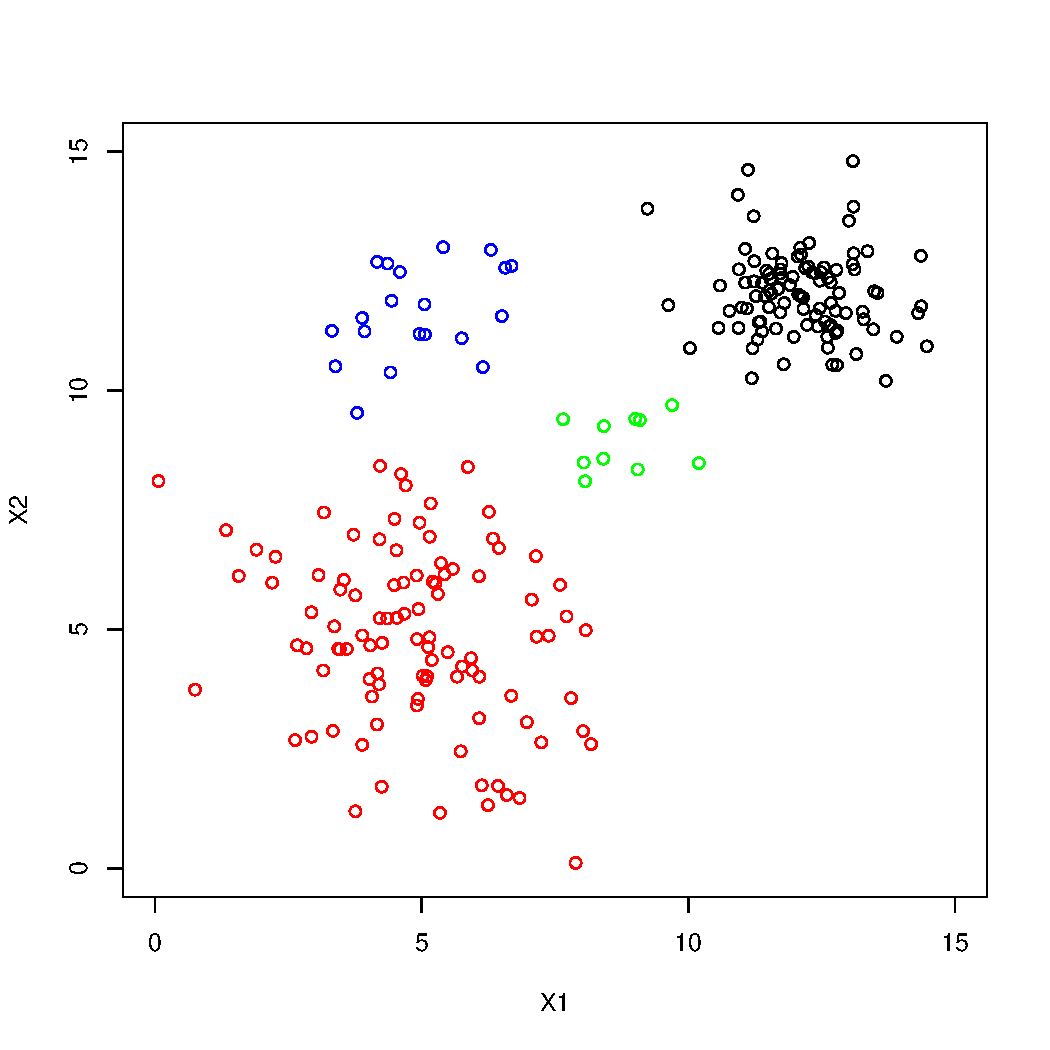
\includegraphics[width=\linewidth]{figure/Data_elbow.pdf}
\end{minipage}
\hspace{0.05in}
\begin{minipage}{0.45\linewidth}
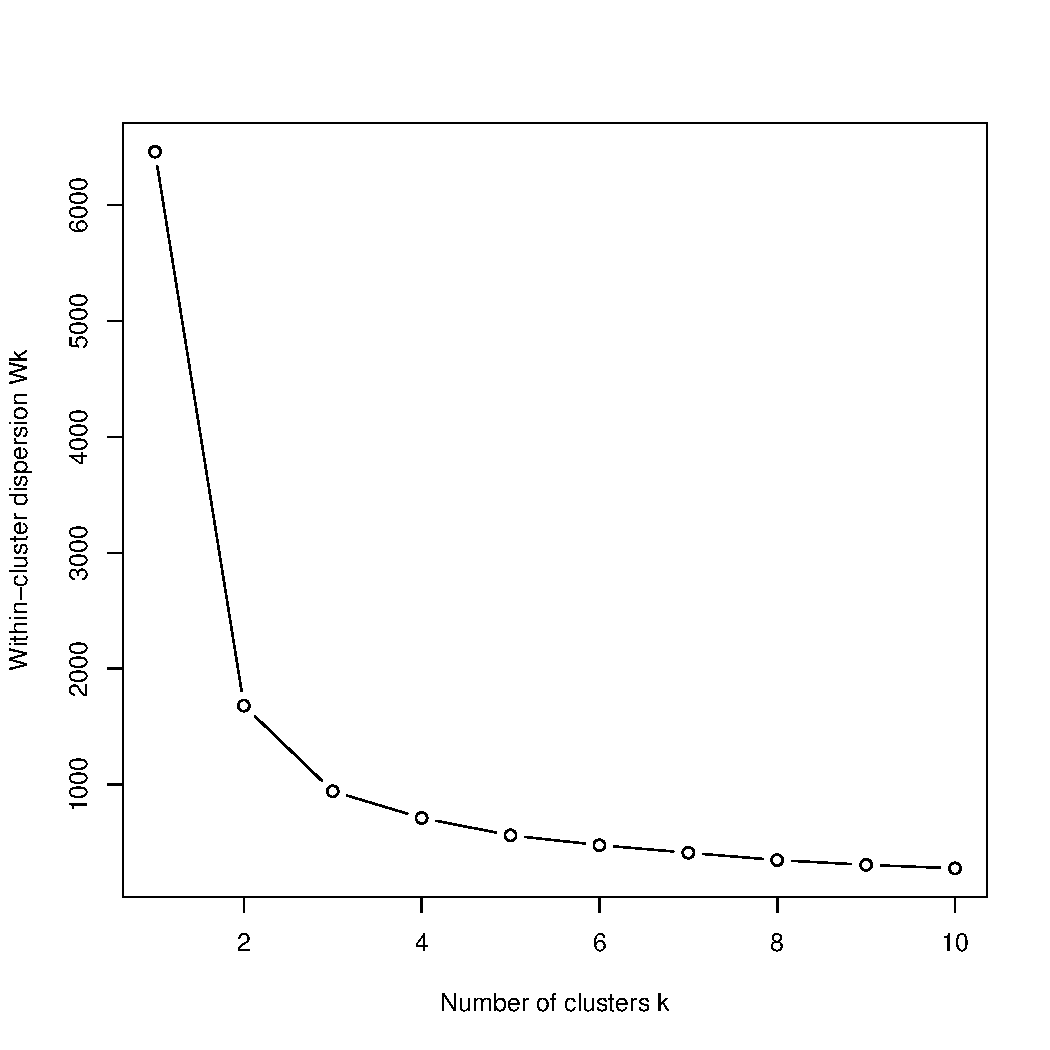
\includegraphics[width=\linewidth]{figure/elbow.pdf}
\end{minipage}
\end{minipage}
\center{\caption{\label{fig1} Left plots show the actual data, right plots show the corresponding $W_k$ \textsl{VS} $k$ curve. }}
\end{figure}
\\

Recently, there are several new proposals to find the $k$ automatically. Gap statistics \citep{tibshirani2001estimating} estimates $k$ by comparing the change in within-cluster dispersion with that expected under an appropriate reference null distribution. Specifically, the graph of $log(W_k)$ is compared with its expectation under an appropriate null reference distribution of the data. The value of $k$ associated with the largest gap between $log(W_k)$ and the reference curve is selected as optimal $k$. \cite{sugar2003finding} proposed an approach which finds the number of clusters based on distortion, a quantity that measures the average distance, per dimension. It's backed by a rigorous theoretical justification based on information-theoretic ideas.   \cite{fraley2002model}'s Model-based method employs the EM algorithm to estimate the parameters in Gaussian mixture model, and select the best model ($k$) using BIC criterion. Stability-based criterion is also proposed to locate the best $k$ by some authors such as \cite{ben2001stability}, \cite{wang2010consistent} and \cite{fang2012selection}. \cite{chiang2010intelligent} provides a nice review of existing methods for finding the right $k$ in published literature. \\

Most existing methods are either model based method requires strong parameter assumptions or ad hoc method utilizes within-cluster dispersion. Although many view selecting the number of clusters as a model selection problem, very few approaches this problem from the prediction point of view. Select model with smallest prediction error via cross-validation is one of the simplest and most widely used model selection techniques in supervised learning. The lack of true class (label) in data set makes the adoption of cross-validation into unsupervised leaning problem difficult. Perhaps the only exception is \cite{tibshirani2005cluster}, which selects the optimal $k$ by prediction strength. The strategy is to first cluster the test data and training data into $k$ clusters respectively. Then, for each pair of observations that are assigned to the same test cluster, algorithm determines whether they are also assigned to the same cluster based on the training centers. The intuition here is, if $k=k_0$, the true number of clusters, then the $k$ training set clusters will be similar to the $k$ test clusters, and hence will predict them well. However, a specifically defined prediction error measure is used in such procedure, which is quite different from the one commonly used in cross-validation procedure in supervised learning. Therefore the well understood properties of cross-validation procedure in supervised learning cannot be carried over to the prediction strength method, makes the interpretation of its result difficult. \\

Our proposed method is a complete data-driven approach which doesn't rely on any parametric assumptions. Trough novel form of partitioning data set, we are able to employing the cross-validation procedure in clustering exactly the same way as in supervised learning problem. Hence, it's easy for reader to understand the intuition behind our proposed method. Simulation and real data application shows the superior performance of our proposed method compare with existing methods in high-dimension settings and heavy-tailed data. Since the embedded cross-validation procedure is well understood, it also makes our method potentially easily to be extended in future study. 
 
\section{Cross-Validation in finding the number of clusters}
Cross-Validation technique, one of the most commonly used and popular model selecting method in supervised learning, can not be used naively in unsupervised learning context. Since prediction error of new observation is calculated by its distance to the nearest cluster center, more cluster centers means much tighter fit to the feature space, and hence smaller distance (prediction error) of observation to its nearest cluster center. This holds even when the prediction is evaluated on an independent test set \citep{hastie2009elements}. Therefore, CV prefers larger $k$ if we do the CV naively.\\

We propose a new strategy to locate the optimal $k$ via Cross Validation. Recall that in supervised leaning, for any CV replicate, we have data in four parts
 $\begin{pmatrix}
  \mathbf{X}_{train} & \mathbf{Y}_{train}\\
  \mathbf{X}_{test}  & \mathbf{Y}_{test}\\
  \end{pmatrix}$.
One builds learner using $\left(\mathbf{X}_{train}, \mathbf{Y}_{train}\right)$ and apply it to $ \mathbf{X}_{test}$ in order to get $\hat{\mathbf{Y}}_{test}$. Difference between $\hat{\mathbf{Y}}_{test}$ and $\mathbf{Y}_{test}$ is measured as prediction error. In unsupervised leaning context, there is no $\mathbf{Y}$, so we only get $\begin{pmatrix}
  \mathbf{X}_{train}\\
  \mathbf{X}_{test}\\
  \end{pmatrix}$. \cite{perry2009cross} considered more general hold-outs in order for cross-validation to work in unsupervised learning. Specifically, two types of hold-outs are considered. The first one is Wold hold-out, which is ``speckled": we leave out random elements of the matrix $\mathbf{X}$ and use missing data algorithm like EM for prediction. The second one is Gabriel hold-out: we randomly partition the columns of $\mathbf{X}$ into ``predictors" and ``response" sets and then perform the CV as in supervised learning. This paper is focused on the Gabriel hold-out, we also developed the Wold hold-out version and included it in the comparison in simulation.  \\\\
We now give the details of how to implement the Gabriel cross-validation to locate the optimal cluster number $k$. The Wold cross-validation algorithm is described in Appendix $A$.

\subsection*{Gabriel CV algorithm}
The basic idea of Gabriel hold-out is to ``create" the label $(Y)$ for data without it, and then perform the cross-validation as in supervised learning. Specifically, given data set 
$\mathbf{X} \in \mathbb{R}^{n \times p}$, we partition it into four parts
\[
\begin{pmatrix}
  \mathbf{X}_{train} & \mathbf{Y}_{train}\\
  \mathbf{X}_{test}  & \mathbf{Y}_{test}\\
  \end{pmatrix} \equiv 
  \begin{pmatrix}
  \mathbf{X}^{m \times q } & \mathbf{X}^{m \times (p-q)}\\
  \mathbf{X}^{(n-m) \times q}  & \mathbf{X}^{(n-m) \times (p-q)}\\
  \end{pmatrix}
 \]
  where $ 1 < m < n$ and $1<q<p$. That is, we leave out $n-m$ rows of data as test set, and make $p-q$ features as ``response". Note that the data set looks like the one in supervised learning now.\\\\
To keep it consistent with the notation used in section $3$, we also denote above partition of data $\mathbf{X}$ as 
\[
\begin{pmatrix}
  \mathbf{X}_{train} & \mathbf{Y}_{train}\\
  \mathbf{X}_{test}  & \mathbf{Y}_{test}\\
  \end{pmatrix} \equiv 
  \begin{pmatrix}
\mathbf{X}^L_{train} & \mathbf{X}^R_{train}\\
  \mathbf{X}^L_{test}  & \mathbf{X}^R_{test}\\
  \end{pmatrix}
 \]
That is, data set $\mathbf{X} \in \mathbb{R}^{n \times p}$ been partitioned in column as $\mathbf{X}^L \in \mathbb{R}^{n \times L}$ and $\mathbf{X}^R \in \mathbb{R}^{n \times R}$, where $\mathbf{X}^L$ is treated as features ($L=q$) and $\mathbf{X}^R$ is treated as response ($R=p-q$).\\
\begin{itemize}
	\item For each $k = 1,2,...,k_{max}$, the Gabriel algorithm works as following
	\begin{enumerate}
 	\item A set of $k$ clusters (labels) $ \mathcal{G}= \{g_1,...,g_k\} $ are returned by applying K-means on $\mathbf{X}^R_{train}$ with parameter $k$, $\hat{\mu}^R \left(g_j\right)$ is the corresponding estimated cluster center for $g_j$, $1 \leq j \leq k$.  
 	\item Train a classifier $\mathcal{C}$ using $\left(\mathbf{X}^L_{train}, \mathcal{G} \right)$. We implement LDA in our algorithm.
 	\item Applying the classifier $\mathcal{C}$ on $\mathbf{X}^L_{test}$, we got a set of predicted clusters $\hat{\mathcal{G}} = \{\hat{g} \left(x^L_i\right) \in \mathcal{G}, i = m+1,...,n \}$, where $\hat{g} \left(x^L_i\right)$ is the predicted (assigned) cluster for observation $x_i$ in the testing data set   
 	\item Calculate the difference between $\hat{\mathcal{G}}$ and  $\mathbf{X}^R_{test}$ as
 	\[Error_k = \sum^n_{i = m+1} ||\hat{g} \left(x^L_i\right) - x^R_i||^2 = \sum^k_{j=1} \sum_{g_j = \hat{g} \left(x^L_i\right)} ||\hat{\mu}^R \left(g_j\right) - x^R_i||^2\]
 	\end{enumerate}
	Note that one can use classification technique other than LDA in step $2.$
\noindent
	\item The algorithm selects $k$ with minimum average $Error_k$ across all CV folds, that is $$\underset{k}{\operatorname{argmin}} \hspace{0.05 in} E\left(Error_k\right) $$
\end{itemize}
\section{Theoretical justification of Gabriel CV method}
This section gives the self-consistency proof of the proposed Gabriel method. What's more, its asymptotic property under suitable condition will be shown in this section in order to give the idea of why the Gabriel CV method works.\\

Because K-means algorithm is a key part in the proof below, it's convenient to have a review of K-means here:\\
Given a set of observations $\mathbf{X} = (x_1,...,x_n)$, and the number of clusters $K$, K-means' goal is to minimize the within cluster dispersion. That is, find the partition $\mathbb{P}_K$ of $\mathbf{X}$, where $\mathbb{P}_K(\mathbf{X})= (p_1,p_2,...,p_K)$, such that
\[	\underset{\mathbb{P}_K}{\operatorname{argmin}} \sum^K_{i=1}\sum_{x \in p_i } ||x-\hat{\mu}_i||^2\]
where $\hat{\mu}_i$ is the sample mean of $p_i$.
\subsection{Self-Consistency}
Same as in section $2$, let the data set $\mathbf{X} \in \mathbb{R}^{n \times p}$ been partitioned as 
 \[ 
 \begin{pmatrix}
\mathbf{X}^L_{train} & \mathbf{X}^R_{train}\\
  \mathbf{X}^L_{test}  & \mathbf{X}^R_{test}\\
  \end{pmatrix}
 \]
\subsection*{Assumptions}
\begin{enumerate}[label={Assumption},leftmargin=*]
\item $1.$ There are $K$ true centers $(\mu_1,...,\mu_K)$ where $\mathbf{X}$ generated from
\item $2.$ The $K$ partitioned centers $(\mu^L_1,...,\mu^L_K)$ are all distinct in $L$ dimensions: $||\mu^L_i-\mu^L_j|| \neq 0$ for any $i \neq j$; $(\mu^R_1,...,\mu^R_K)$ are all distinct in $R$ dimensions
\item $3.$ The training set contains at least one member of each cluster
\item $4.$ The test set contains at least one member of each cluster
\item $5.$ There is no noise, so that $$x_i = \mu \left(c_i\right) \in \{\mu_1,...,\mu_K\} $$ and $$\mu \left(c_i\right) = \mu_j \hspace{0.2in} \text{iff} \hspace{0.2in} c_i = j$$ where $c_i$ is the true cluster for observation $i$, which implies $$x^L_i = \mu^L\left(c_i\right) \in \{\mu^L_1,...,\mu^L_K\},\hspace{0.2in} x^R_i = \mu^R\left(c_i\right) \in \{\mu^R_1,...,\mu^R_K\}$$
\end{enumerate}
 
\begin{proposition}
	If assumptions $1, 2, 3, 5$ hold, then there exists a classification method works perfectly in case of ($k \leq K$): the re-substitution error is $0$. That is, for $\forall x_i \in \mathbf{X}_{train}$ prediction on $x^L_i$ always correctly predict cluster where $x^R_i$ is in.
\end{proposition}

\begin{theorem}
Given assumptions $1-5$, $ E\left(Error_k\right) > 0$ for $k<K$ and  $ E\left(Error_k\right) = 0$ for $k=K$. Hence if $k \leq K$, the Gabriel algorithm selects $k=K$ with probability $1$.
\end{theorem}
\noindent
Not that $k > K$ is not considered here because there are only $K$ unique points in $\mathbf{X}$. K-means will not work for parameter which is larger than the number of unique points in data $\mathbf{X}$.\\\\ 
\noindent
The proof of above theorem follows from following two lemmas:
\begin{lemma}
	If the assumptions of Theorem $1$ hold, then when $k<K$, the CV Error $>0$
\end{lemma}
\begin{proof}
	It is sufficient to prove that when $k<K$,  $Error_k>0$. By the definition of $Error_k$,
\begin{equation}
Error_k = \sum^k_{j=1} \sum_{g_j = \hat{g} \left(x^L_i\right)} ||\hat{\mu}^R \left(g_j\right) - x^R_i||^2
\end{equation}
	where $\hat{\mu}^R \left(g_j\right)$ is the center of cluster $g_j$ returned from K-means. By assumption $4$, test set contains at least one member of each cluster. Since there are $K$ true centers, and by assumption $5$, $x_i = \mu \left(c_i\right) \in \{\mu_1,...,\mu_K\} $, test set contains $K$ centers. It means there are $K$ distinct $x^R_i \left(=\mu^R \left(c_i\right)\right)$ in $\mathbf{X}^R_{test}$ set by assumption $2$. However, in equation $(1)$, there are only $k$ distinct $\hat{\mu}^R \left(g_j\right)$.  Because $k < K$, it means not every element $||\hat{\mu}^R \left(g_j\right) - x^R_i||^2 = 0$ in equation $(1)$. Therefore,  $$Error_k = \sum^k_{j=1} \sum_{g_j = \hat{g} \left(x^L_i\right)} ||\hat{\mu}^R \left(g_j\right) - x^R_i||^2 > 0$$
\end{proof}
\begin{lemma}
	If the assumptions of Theorem $1$ hold, when $k=K$, the CV Error $=0$
\end{lemma}
\begin{proof}
	It's sufficient to show that when $k=K$, $Error_k=0$. By assumption $3$ and $5$, training set contains $K$ centers. Which also implies $\mathbf{X}^R_{train}$ contains $K$ distinct $x^R_i$ $(\mu^R_1,...,\mu^R_K)$. When apply K-means on $\mathbf{X}^R_{train}$ with parameter $K$, the unique solution of 
	\[ \underset{\left(\hat{\mu}^R\left(g_1\right),...,\hat{\mu}^R\left(g_K\right)\right)}{\operatorname{argmin}} \sum^K_{j=1} \sum_{g_j = \hat{g} \left(x^R_i\right)} ||\hat{\mu}^R \left(g_j\right) - x^R_i||^2 \]
	is 
\begin{equation}	
	\{\hat{\mu}^R \left(g_j\right) = \mu^R_j, j=1,...,K\}
\end{equation}	
with 
\begin{equation}	 
	\hat{g} \left(x^R_i\right) = \sum^K_{j=1} g_j \cdot I_{c_i = j}
\end{equation}	
Where $\hat{g} \left(x^R_i\right) \in  \mathcal{G}$ is the assigned cluster of $x^R_i$ by K-means. One can easily check that such solution is unique and above objective function attains its lower bound $0$.\\\\
By Proposition $1$, $\mathcal{C}$ has re-substitution error $0$, which means its prediction error is $0$ on $\mathbf{X}^L_{test}$ as $\forall x^L_i \in \mathbf{X}^L_{test}, x^L_i \in \mathbf{X}^L_{train}$ by assumption $1,3,5$. Hence the predicted cluster $\hat{g} \left(x^L_i\right)$ for $x_i$ is the correct one $\hat{g} \left(x^R_i\right)$, which determined by $x^R_i$. By equation $(3)$, we have $x^R_i = \mu^R \left(c_i\right) = \mu^R_j$ if $\hat{g} \left(x^L_i\right) = \hat{g} \left(x^R_i\right) = g_j$. Therefore,
\[ Error_K = \sum^K_{j=1} \sum_{g_j = \hat{g} \left(x^L_i\right)} ||\hat{\mu}^R \left(g_j\right) - x^R_i||^2 =  \sum^K_{j=1} \sum_{g_j = \hat{g} \left(x^L_i\right)} ||\hat{\mu}^R \left(g_j\right) - \mu^R_j||^2= 0\]
The last equation holds because of equation $(2)$.
\end{proof}

\begin{itemize}
	\item Proof of \textbf{Proposition} $1$.
	\begin{proof}
	To train classifier $\mathcal{C}$, we have training set $\left(\mathbf{X}^L_{train},\mathcal{G} \right) = \{\left(x^L_i,\hat{g} \left(x^R_i\right)\right), i =1,2,...,m\}$. By assumption $5$, $\forall i$ $x_i = \mu_j$, $j=1,2,...,K$ and $k \leq K$. Hence the training set has $K$ unique pairs $\{\left(\mu^L_j, \hat{g} \left(\mu^R_j\right)\right),j=1,2,...,K\}$, with $K$ unique $\mu^L_j$ by assumption $3$ and $k$ unique $\hat{g} \left(\mu^R_j\right)$. This is because each pair $(\mu^L_j,\mu^R_j)$ is unique by assumption $2$ and $\left(\mu^R_j,\hat{g} \left(\mu^R_j\right)\right)$ is unique since K-means assigns one and only one label to each $\mu^R_j$. Define the classifier $\mathcal{C}$ as following: \[ \mathcal{C}(x^L_i) = \sum^K_{j=1}\hat{g} \left(\mu^R_j\right) \cdot I_{\{c_i = j\}}  \] It's easy to see such classifier has re-substitution error $0$. 
	\end{proof}
	\item Proof of \textbf{Proposition} $1$ when the classifier is LDA.
	\begin{proof}
	Since Proposition $1$ is only used in Lemma $2$, therefore it's sufficient to prove it in case of $k = K$. Note that training set contains $K$ unique pairs $\{\left(\mu^L_j, \hat{g} \left(\mu^R_j\right)\right), j=1,2,...,K\}$, with $K$ unique $\mu^L_j$ and $K$ unique $\hat{g} \left(\mu^R_j\right)$ now, where $\mu^L_j, \hat{g} \left(\mu^R_j\right)$ has one-to-one correspondence, i.e.
\[ \left\lbrace\left(\mu^L_j,\hat{g} \left(\mu^R_j\right) \right), j=1,2,...,K\right\rbrace =  \left\lbrace\left(\mu^L_j, g_j \right), j=1,2,...,K\right\rbrace \]
By equation $(3)$.\\\\
Let the prior probability of class $g_j$ be $\pi_j, \hspace{0.05in} j=1,...,K$. By assumption $3$, $\pi_j > 0$. The class-conditional density of $X$ in class $\mathcal{G} = g_j$ is $$f_j\left(x_i\right) = \mathbb{P}\left( X=x_i | \mathcal{G} = g_j \right) $$ where $x_i \in \{\mu^L_1,...,\mu^L_K\}$ and $f_j\left(x_i\right)$ has multivariate Gaussian distribution
\[ f_j\left(x_i\right) = \frac{1}{(2\pi)^{p/2}|\Sigma_j|^{1/2}}e^{-\frac{1}{2}(x_i-\mu_j)^T\Sigma^{-1}_j(x_i-\mu_j)	}\]
LDA assumes a commom covariance matrix $\Sigma_j = \Sigma \hspace{0.1in} \forall j$.
The posterior probability is 
\[	\mathbb{P}\left( \mathcal{G} = g_j | X=x_i  \right)  = \frac{f_j\left(x_i\right) \pi_j}{\sum^K_{l=1}f_l\left(x_i\right) \pi_l}	\]
In practice, $\pi_j, \mu_j$ and $\Sigma$ are estimated from data by
 \begin{itemize}
 	\item  $\hat{\pi}_j = \frac{N_j}{N}$, where $N_j$ is the number of class-$g_j$ observation in training set and $N$ is the total observation in training set
 	\item  $\hat{\mu}_j = \sum_{c_i=j} x_i/N_j$ 
 	\item  $\hat{\Sigma} = \frac{1}{N-K} \sum^K_{j=1}\sum_{c_i=j} (x_i - \hat{\mu}_j )(x_i - \hat{\mu}_j )^T$
 \end{itemize}
In our case, $\hat{\mu}_j = \mu^L_j$ and $\hat{\Sigma}$ is zero matrix by construction. But in real case, the estimate of within-group covariance $\hat{\Sigma}$ is a positive-definite matrix. We therefore assume $\hat{\Sigma}$ to be any positive-definite matrix. Also, we assume the observations in training set are evenly distributed across all class, i.e. $\pi_j$ is a positive constant for all $j = 1,...,K$ \\\\   
LDA predicts class for each $x_i = \mu^L(c_i)\in \{\mu^L_1,...,\mu^L_K\}$ by maximizing the posterior probability
\begin{align}
     \hat{\mathcal{G}}(x_i) & = \underset{g_j}{\operatorname{argmax}}\hspace{0.05 in} \mathbb{P}\left( \mathcal{G} = g_j | X=x_i  \right)  \nonumber   \\ 
     & = \underset{g_j}{\operatorname{argmax}}\hspace{0.05 in} f_j\left(x_i\right) \pi_j \nonumber \nonumber  \\
     & = \underset{g_j}{\operatorname{argmax}}\hspace{0.05 in} f_j\left(x_i\right) \nonumber  \nonumber  \\    
     & = \underset{g_j}{\operatorname{argmax}}\hspace{0.05 in}  \frac{1}{(2\pi)^{p/2}|\hat{\Sigma}|^{1/2}}e^{-\frac{1}{2}(x_i-\mu^L_j)^T\hat{\Sigma}^{-1}(x_i-\mu^L_j)	} \nonumber  \\  
     &=  \underset{g_j}{\operatorname{argmin}}\hspace{0.05 in} (x_i-\mu^L_j)^T\hat{\Sigma}^{-1}(x_i-\mu^L_j) \nonumber   \\  
     &= \sum^K_{j=1} g_j \cdot I_{c_i = j}
\end{align}
The last equation holds because $\hat{\Sigma}$ is assumed to be positive-definite, so is its inverse  $\hat{\Sigma}^{-1}$. Hence $(x_i-\mu^L_j)^T\hat{\Sigma}^{-1}(x_i-\mu^L_j) >0$ for any non-zero vector $(x_i-\mu^L_j)$. The lower bound $0$ is attained only when $(x_i-\mu^L_j)$ is a zero vector, which is only possible when $x_i=\mu^L(c_i) = \mu^L_j$, i.e. $c_i = j$ by assumption $2$ and $5$. \\\\
Because the RHS of equation $(4)$ coincide with RHS of equation $(3)$, the proof is complete.
\end{proof}
\end{itemize}
\subsection{Well-separated clusters with noise}
Same with previous, the data set $\mathbf{X} \in \mathbb{R}^{n \times p}$ been partitioned as $\mathbf{X}^L \in \mathbb{R}^{n \times L}$ and $\mathbf{X}^R \in \mathbb{R}^{n \times R}$, with following set of assumptions:
\begin{enumerate}[label={Assumption},leftmargin=*]
	\item $1.$ There are $K$ true centers $(\mu_1,...,\mu_K)$ where $\mathbf{X}$ generated from
	\item $2.$ The $K$ partitioned centers $(\mu^L_1,...,\mu^L_K)$ are all distinct in $L$ dimensions: $||\mu^L_i-\mu^L_j|| \neq 0$ for any $i \neq j$; $(\mu^R_1,...,\mu^R_K)$ are all distinct in $R$ dimensions
	\item $3.$ There is noise, i.e. $$x_i = \mu \left(c_i\right) + \varepsilon_i, \hspace{0.2 in} \mu \left(c_i\right) \in \{\mu_1,...,\mu_K\}$$ where vector $\varepsilon_i$ is i.i.d with zero mean and covariance matrix $\Sigma$, which is independent from any $\mu_j \in (\mu_1,...,\mu_K)$, $c_i$ is the true cluster for observation $i$, which implies $$x^L_i = \mu^L \left(c_i\right) + \varepsilon^L_i,\hspace{0.2in} x^R_i = \mu^R \left(c_i\right) + \varepsilon^R_i$$ 
with $$\mu^L\left(c_i\right) \in \{\mu^L_1,...,\mu^L_K\},\hspace{0.2in} \mu^R\left(c_i\right) \in \{\mu^R_1,...,\mu^R_K\} $$\
where $\varepsilon^L_i$ and $\varepsilon^R_i$ are independent and both have zero mean and covariance matrix $\Sigma^L$ and $\Sigma^R$ respectively, so $\Sigma = 
\begin{pmatrix}
  \Sigma^L &0\\
  0  &\Sigma^R\\
  \end{pmatrix}$
. Also $\varepsilon^R_i$ is bounded $||\varepsilon^R_i|| \leq 1$.
	\item $4.$ Clusters are well separated, i.e. \[ ||x_i-\mu \left(c_i\right)|| < ||x_i-\mu_{j}|| \hspace{0.2 in}\forall \hspace{0.01 in}j\neq c_i \] and \[ ||x^L_i-\mu^L \left(c_i\right)|| < ||x^L_i-\mu^L_{j}||-\delta,  \hspace{0.2 in}||x^R_i-\mu^R \left(c_i\right)|| < ||x^R_i-\mu^R_{j}||-\delta \hspace{0.2 in}\forall \hspace{0.01 in}j\neq c_i\] where $\delta > 0$ is a small constant 
	\item $5.$ The training set contains $n^{train}_j>0$ observations from each cluster $j$ and the test set contains $n^{test}_j > 0$ observations from each cluster $j$, $j=1,2...,K$
	\item $6.$ The prior for $x_i$ come from cluster $\mu_j$ is $\pi_j > 0$. So when the total number of observation in training set $m$ goes infinity, $\lim_{m\to \infty} n^{train}_j = m \cdot \pi_j $. Also $m=n\cdot r$, $n-m = n\cdot (1-r)$, where $0<r<1$ is a positive constant.
\end{enumerate}

\subsubsection{Consistent assumption for K-means}
\cite{pollard1981strong} found conditions that ensure the almost sure convergence of the set of cluster centers of K-means as the sample size increase. This section mainly introduce the theorem from \cite{pollard1981strong} and show the assumptions needed for our own theorem.\\\\  
Applying K-means clustering on i.i.d observations $x_1,x_2,...x_m$ from population $P$ with parameter $k$ is to choose cluster centers $a_1,a_2,...,a_k$ to minimize
\[	W_m = \frac{1}{m}\sum^m_{l=1}min_{1\leq j \leq k}||x_l-a_j||^2	\]
It's convenient to treat $W_m$ as a function of the set of cluster centers $A$ and of the  empirical distribution $P_m$ obtained from the sample by placing mass $m^{-1}$ at each of $x_1,x_2,...x_m$. Then the problem is to minimize 
\[ W(A,P_m):=\int min_{a\in A}||x-a||^2P_m(dx)\]
Over all possible choices of the set $A$ containing $k$ points. \\\\
For each probability measure $Q$ and each set $A$, defined
\[	\Phi(A,Q):= \int min_{a\in A}||x-a||^2 Q(dx)	\] and \[ \mathfrak{m}_k(Q):=inf\{\Phi(A,Q):A \hspace{0.05in} \text{contains} \hspace{0.05in} k  \hspace{0.05in} \text{or fewer points}\} \]
The theorem proved by \cite{pollard1981strong} says that
\begin{theorem}
	Suppose that $\int ||x||^2P(dx) < \infty$ and that for each $j=1,2,...,k$ there is a unique set $\bar{A}(j)$ for which $\Phi(\bar{A}(j),P)=\mathfrak{m}_j(P)$. Then $A_m \to \bar{A}(k)$ a.s and $\Phi(A_m,P_m) \to \mathfrak{m}_k(P)$ a.s 
\end{theorem}
\noindent
Where $A_m = A_m(k)$ is the set of optimal sample cluster centers satisfy $\Phi(A_m,P_m) = \mathfrak{m}_k(P_m)$ and $\bar{A}=\bar{A}(k)$ is the set of optimal population cluster center satisfy  $\Phi(\bar{A},P) = \mathfrak{m}_k(P)$. Such theorem gives the condition for the sample estimator of cluster centers be consistent estimator of optimal cluster centers.\\

In our setting, observations $x^R_1, x^R_2,...,x^R_m$ can be viewed as i.i.d observations from same distribution $\mathcal{P}$, which is a mixed distribution of $K$ distinct distributions with prior $\pi_1,\pi_2,...,\pi_K$.
\begin{theorem}
Suppose assumption $3$ holds and for each $j=1,2,...,k_{max}$ there is a unique set $\bar{A}(j)$ for which $\Phi(\bar{A}(j),\mathcal{P})=\mathfrak{m}_j(\mathcal{P})$, also $ \bar{A}(K) = \{\mu^R_1,\mu^R_2,...,\mu^R_K\}$. Then for any $k \leq k_{max}$, $A_m(k) \to \bar{A}(k)$ a.s.
\end{theorem}
\begin{proof}
By assumption $3$, $||\varepsilon^R_i||\leq 1$, which implies the first condition in theorem $2$ holds, i.e.
\[\int ||x||^2P(dx) < \infty\] 
Since the second condition of theorem $2$ is given as assumption in theorem $3$, we have almost sure convergence of cluster centers $A_m(k)$ for any $k \leq k_{max}$ by theorem $2$. 
\end{proof}
\noindent
In the rest of this section, the assumptions (conditions) given in theorem $3$ is called consistent assumptions. 
\subsubsection{Asymptotic property of Gabriel method}
\begin{definition}
Define event\\ $\mathcal{D} = \{\forall x_i \in \mathbf{X}, ||x^L_i-\hat{\mu}^L \left(c_i\right)|| < ||x^L_i-\hat{\mu}^L_{j}||, ||x^R_i-\hat{\mu}^R \left(c_i\right)|| < ||x^R_i-\hat{\mu}^R_{j}|| \hspace{0.2 in} \forall \hspace{0.01 in}j\neq c_i\}$, where $\hat{\mu}^R_{j}$ is the sample mean of $j^{th}$ cluster in $\mathbf{X}^R_{train}$and $\hat{\mu}^L_{j}$ is the sample mean of $j^{th}$ cluster in $\mathbf{X}^L_{train}$
\end{definition}

\begin{proposition}
Under assumptions $1-6$, $P(\mathcal{D}) \to 1$ with $m \to \infty$.
\end{proposition}
\begin{proof}
	By assumption $4$, \[  ||x^L_i-\mu^L \left(c_i\right)|| < ||x^L_i-\mu^L_{j}||-\delta \hspace{0.2in} \forall \hspace{0.01 in}j\neq c_i \] 
	Hence, 
	\begin{align} \nonumber
		||x^L_i-\hat{\mu}^L \left(c_i\right)|| & \leq \nonumber ||x^L_i-\mu^L \left(c_i\right)||+ ||\mu^L \left(c_i\right)-\hat{\mu}^L \left(c_i\right) ||\\ \nonumber
		&< ||x^L_i-\mu^L_{j}||-\delta + ||\mu^L \left(c_i\right)-\hat{\mu}^L \left(c_i\right) ||  \\ \nonumber
		& \leq ||x^L_i-\hat{\mu}^L_{j}||+||\mu^L_{j}-\hat{\mu}^L_{j}||-\delta + ||\mu^L \left(c_i\right)-\hat{\mu}^L \left(c_i\right) ||  \\ \nonumber
		& =  ||x^L_i-\hat{\mu}^L_{j}||-\left\lbrace \delta-||\mu^L_{j}-\hat{\mu}^L_{j}|| -||\mu^L \left(c_i\right)-\hat{\mu}^L \left(c_i\right) || \right\rbrace \\ 
m \to \infty		&<||x^L_i-\hat{\mu}^L_{j}||
	\end{align} 
The step $(5)$ is because for any given $\varepsilon > 0$, by Markov inequality
	\begin{align} \nonumber
	  P\left(||\mu^L_{j}-\hat{\mu}^L_{j}||^2 \geq \varepsilon \right) &\leq \frac{E||\mu^L_{j}-\hat{\mu}^L_{j}||^2}{\varepsilon}  \nonumber \\ \nonumber
	    &=  \frac{E\left(\mu^L_{j}-\hat{\mu}^L_{j}\right)^T\left(\mu^L_{j}-\hat{\mu}^L_{j}\right)}{\varepsilon}  \\ \nonumber
	    &=  \frac{E[ tr\left\lbrace\left(\mu^L_{j}-\hat{\mu}^L_{j}\right)^T\left(\mu^L_{j}-\hat{\mu}^L_{j}\right)\right\rbrace]}{\varepsilon}  \\ \nonumber
	   &=  \frac{E[ tr\left\lbrace\left(\mu^L_{j}-\hat{\mu}^L_{j}\right)\left(\mu^L_{j}-\hat{\mu}^L_{j}\right)^T\right\rbrace]}{\varepsilon}  \\ \nonumber
	  &=  \frac{ tr\left\lbrace E\left(\mu^L_{j}-\hat{\mu}^L_{j}\right)\left(\mu^L_{j}-\hat{\mu}^L_{j}\right)^T\right\rbrace}{\varepsilon}  \\ \nonumber
	  &= \frac{ tr\{\Sigma^L \}}{n^{train}_j \cdot \varepsilon}   \\ \nonumber
	% \lim_{m\to \infty} n^{train}_j = m \cdot \pi_j \to \infty \hspace{1in} &\to 0  \\ \nonumber
	\end{align} 
So
\begin{align} \nonumber
  max_{j \in \{1,2,...,K\}} \hspace{0.05in} P\left(||\mu^L_{j}-\hat{\mu}^L_{j}||^2 \geq \varepsilon \right) &\leq max_{j \in \{1,2,...,K\}} \hspace{0.05in}\frac{E||\mu^L_{j}-\hat{\mu}^L_{j}||^2}{\varepsilon}  \nonumber \\ \nonumber
  &=max_{j \in \{1,2,...,K\}} \hspace{0.05in}  \frac{ tr\{\Sigma^L \}}{n^{train}_j \cdot \varepsilon}   \\ \nonumber
m \to \infty \hspace{0.3in}  &= \frac{ tr\{\Sigma^L \}}{m\hspace{0.02in}\pi^*\hspace{0.02in} \varepsilon}  \hspace{0.5in} \text{where}\hspace{0.1in}\pi^* = min_{j \in \{1,2,...,K\}}\pi_j\\ \nonumber
&\to 0
\end{align} 

Therefore $\forall j, \hspace{0.05in} ||\mu^L_{j}-\hat{\mu}^L_{j}|| \to 0$ uniformly as $m \to \infty$. Hence, 
\begin{equation}
\lim_{m\to \infty} \left\lbrace \delta-||\mu^L_{j}-\hat{\mu}^L_{j}|| -||\mu^L \left(c_i\right)-\hat{\mu}^L \left(c_i\right) || \right\rbrace >0
\end{equation}

Same argument yields 
\[||x^R_i-\hat{\mu}^R \left(c_i\right)|| < ||x^R_i-\hat{\mu}^R_{j}||\]
Because $(6)$ holds uniformly $\forall j\in\{1,2,...,K\}$, we have 
\[ \lim_{m \to \infty}P(\mathcal{D})  =1\]
	\end{proof}
\begin{proposition}
Given assumption $1-6$ and the consistent assumptions of Theorem $3$, when $m \to \infty$, $P\left[A_m(K) = \{\hat{\mu}^R_1,\hat{\mu}^R_2,...,\hat{\mu}^R_K \}\right]=1$, where $\hat{\mu}^R_j$ is the sample mean of $j^{th}$ cluster in $\mathbf{X}^R_{train}$
\end{proposition}
\begin{proof}
By theorem $3$, we know $A_m(K) \to \bar{A}(K)$ a.s. and $\bar{A}(K) = \{\mu^R_1,\mu^R_2,...,\mu^R_K\}$. Denote $A_m(K) = \{a_1, a_2,..., a_K\}$, by almost sure convergence of $A_m(K)$ to $\bar{A}(K)$, we have\\\\
For all $\varepsilon > 0$, there exists $N_{\varepsilon}$ such that if $m > N_{\varepsilon}$, then
\[ P\left(||a_j-\mu^R_j||< \varepsilon\hspace{0.1in}\forall j\right)=1\]
 Now, take $\varepsilon = \frac{\delta}{2}$, then exists $N_{\delta}$ such that for all $m > N_{\delta}$
\[P\left(||a_j-\mu^R_j||<\frac{\delta}{2} \hspace{0.1in}\forall j\right)=1\]
By assumption $4$, 
\[||x^R_i-\mu^R \left(c_i\right)|| < ||x^R_i-\mu^R_{j}||-\delta \hspace{0.2 in}\forall \hspace{0.01 in}j\neq c_i\]
Let $m > N_{\delta}$, for all $x^R_i \in \mathbf{X}^R_{train}$, with probability $1$

\begin{align}
  ||x^R_i - a(c_i)||&\leq ||x^R_i-\mu^R(c_i)|| + ||\mu^R(c_i)-a(c_i)||\nonumber \\ \nonumber
   &< ||x^R_i-\mu^R_{j}||-\delta + ||\mu^R(c_i)-a(c_i)|| \hspace{0.2 in} \forall \hspace{0.01 in}j\neq c_i  \\ \nonumber
    &\leq ||x^R_i-a_{j}|| + ||a_j - \mu^R_{j}||-\delta + ||\mu^R(c_i)-a(c_i)||  \\ \nonumber
 ||\mu^R(c_i)-a(c_i)||< \frac{\delta}{2} \hspace{0.05in}\& \hspace{0.05in}||a_j - \mu^R_{j}||< \frac{\delta}{2} \hspace{0.2in} &<||x^R_i-a_{j}||\hspace{0.2 in}  \forall \hspace{0.01 in}j\neq c_i 
\end{align}
Hence, $x^R_i$ is assigned to cluster center $a(c_i)$ by K-means. Note also that observations from same cluster are assigned to the same center. Since $a_j$ is the sample mean of all the observations assigned to it, we have
\[a_j = \hat{\mu}^R_j \hspace{0.1in}\forall j\]
 where $\hat{\mu}^R_j$ is the sample mean of $j^{th}$ cluster in $\mathbf{X}^R_{train}$. The proof is complete.
\end{proof}
\begin{proposition}
Conditioning on $\mathcal{D}$ and $A_m(K) = \{\hat{\mu}^R_1,\hat{\mu}^R_2,...,\hat{\mu}^R_K \}$, there exists a classification method works perfectly in case of $k = K$: the prediction error is $0$. That is, $\forall x_i \in \mathbf{X}_{test}$ prediction on $x^L_i$ always correctly predict cluster where $x^R_i$ is in. 
\end{proposition}

\begin{proof}
Given $A_m(K) = \{\hat{\mu}^R_1,\hat{\mu}^R_2,...,\hat{\mu}^R_K \}$,  we know from the proof of proposition $3$ that when applying K-means on $\mathbf{X}^R_{train}$ with parameter $K$, the solution of
\[ \underset{\left(\hat{\mu}^R\left(g_1\right),...,\hat{\mu}^R\left(g_K\right)\right)}{\operatorname{argmin}} \sum^K_{j=1} \sum_{g_j = \hat{g} \left(x^R_i\right)} ||\hat{\mu}^R \left(g_j\right) - x^R_i||^2 \]
is 
\begin{equation}
\{\hat{\mu}^R\left(g_j\right) = \hat{\mu}^R_{j}, j=1,...,K\}
\end{equation}
with 
\begin{equation}
\hat{g} \left(x^R_i\right) = \sum^K_{j=1} g_j \cdot I_{c_i = j}
\end{equation}
where $\hat{g} \left(x^R_i\right)$ is the assigned cluster by K-means for observation $x^R_i \in \mathbf{X}^R_{train}$  , $\hat{\mu}^R\left(g_j\right)$ is the sample mean (centroid) of K-means returned cluster $g_j$, $\hat{\mu}^R_{j}$ is the sample mean of $j^{th}$ cluster in $\mathbf{X}^R_{train}$, $c_i$ is the true cluster for observation $i$.\\\\
The training set of $\mathcal{C}$ consists of data in the form of 
\[
\left(\mathbf{X}^L_{train},\mathcal{G} \right) = \left\lbrace \left(x^L_i,\hat{g} \left(x^R_i\right)\right)\right\rbrace, \hspace{0.2in} i =1,2,...,m
 \]
From $(8)$, we learned that observations from the same cluster have been clustered together in the training set. 
And if $g_j = \hat{g} \left(x^R_i\right)$ for observation $i$
\[x^R_i = \mu^R \left(c_i\right) + \varepsilon^R_i = \mu^R_{j} + \varepsilon^R_i\] 
Which implies  
\[x^L_i = \mu^L \left(c_i\right) + \varepsilon^L_i = \mu^L_{j} + \varepsilon^L_i\] 
Hence training set of $\mathcal{C}$ consists of data in the form of 
\[ \left(\mathbf{X}^L_{train},\mathcal{G} \right) = \left\lbrace\left(\mu^L_{j} + \varepsilon^L_i, g_j \right)\right\rbrace\hspace{0.2in} j =1,2,...,K, \hspace{0.1in} i=1,...,m\]
So Let $\hat{\mu}^L_{j} = \frac{\sum x^L_i \cdot I_{c_i=j} }{n^{train}_j}$, $x^L_i  \in \mathbf{X}^L_{train}$ denotes the sample mean of each cluster in $\mathbf{X}^L_{train}$. Define following classifier
	 \[ \mathcal{C}(x^L_i) = \sum^K_{j=1} g_j \cdot I_{h(i) = j} \]
	 where\[h(i) = \underset{j}{\operatorname{argmin}} \hspace{0.05 in}||x^L_i - \hat{\mu}^L_j|| \]
	Note here $x^L_i  \in \mathbf{X}^L_{test}$.\\
	
Then, above classifier has prediction error $0$. To prove it, we need to show above classifier $\mathcal{C}(x^L_i)$ always gives the same cluster as the one in equation $(8)$, i.e. 
\begin{equation}
\mathcal{C}(x^L_i) = \sum^K_{j=1} g_j \cdot I_{c_i = j}
\end{equation}
Given $\mathcal{D}$, we have
\[||x^L_i-\hat{\mu}^L \left(c_i\right)|| < ||x^L_i-\hat{\mu}^L_{j}||\hspace{0.2 in}\forall \hspace{0.01 in}j\neq c_i\]
Which means
\[h(i) = \underset{j}{\operatorname{argmin}} \hspace{0.05 in}||x^L_i - \hat{\mu}^L_j|| = c_i \]
$(9)$ follows directly.
\end{proof}
\noindent
If we further assume equal prior are observed in training set, then we can show that the LDA classifier has prediction error $0$, that is
\begin{proposition}
Conditioning on $\mathcal{D}$ and $A_m(K) = \{\hat{\mu}^R_1,\hat{\mu}^R_2,...,\hat{\mu}^R_K \}$ and $n^{train}_j=\frac{m}{K}$ $\forall j$ in training set, the classifier $\mathcal{C}$ trained using LDA has prediction error $0$ in case of $k = K$.
\end{proposition}
\begin{proof}
Same as in the proof of proposition $4$, given $A_m(K) = \{\hat{\mu}^R_1,\hat{\mu}^R_2,...,\hat{\mu}^R_K \}$, the training set of $\mathcal{C}$ consists of data in the form of 
\[ \left(\mathbf{X}^L_{train},\mathcal{G} \right) = \left\lbrace\left(\mu^L_{j} + \varepsilon^L_i, g_j \right)\right\rbrace\hspace{0.2in} j =1,2,...,K, \hspace{0.1in} i=1,...,m\]
The class-conditional density of $X^L$ in class $\mathcal{G} = g_j$ is $$f_j\left(x^L_i\right) = \mathbb{P}\left( X^L=x^L_i | \mathcal{G} = g_j \right) $$ where $x^L_i=\mu^L(c_i)+\varepsilon^L_i$ and $f_j\left(x^L_i\right)$ has multivariate Gaussian distribution
\[ f_j\left(x^L_i\right) = \frac{1}{(2\pi)^{L/2}|\Sigma^L_j|^{1/2}}e^{-\frac{1}{2}(x^L_i-\mu^L_j)^T(\Sigma^L_j)^{-1}(x^L_i-\mu^L_j)	}\]
LDA assumes a commom covariance matrix $\Sigma^L_j = \Sigma^L \hspace{0.1in} \forall j$.
The posterior probability is 
\[	\mathbb{P}\left( \mathcal{G} = g_j | X^L=x^L_i  \right)  = \frac{f_j\left(x^L_i\right) \pi_j}{\sum^K_{l=1}f_l\left(x^L_i\right) \pi_l}	\]
where $ \pi_j$ is the prior for class $g_j$. In practice, $\pi_j, \mu^L_j$ and $\Sigma^L$ are estimated from data by
 \begin{itemize}
 	\item  $\hat{\pi}_j = \frac{n^{train}_j}{m}$, where $n^{train}_j$ is the number of class-$g_j$ observation in training set and $m$ is the total observations in training set
 	\item  $\hat{\mu}^L_{j} = \frac{\sum x^L_i \cdot I_{c_i=j} }{n^{train}_j}$, $x^L_i  \in \mathbf{X}^L_{train}$
 	\item  $\hat{\Sigma}^L = \frac{1}{m-K} \sum^K_{j=1}\sum_{c_i=j} (x^L_i - \hat{\mu}^L_j )(x^L_i - \hat{\mu}^L_j )^T$
 \end{itemize}
Because $\forall j$ $n^{train}_j=\frac{m}{K}$ , $\hat{\pi}_j = \frac{1}{K}$ $\forall j$. LDA predicts class for each $x^L_i  \in \mathbf{X}^L_{test}$ by maximizing the posterior probability
\begin{align}
     \hat{\mathcal{G}}(x_i) & = \underset{g_j}{\operatorname{argmax}}\hspace{0.05 in} \mathbb{P}\left( \mathcal{G} = g_j | X^L=x^L_i  \right)  \nonumber   \\ 
     & = \underset{g_j}{\operatorname{argmax}}\hspace{0.05 in} f_j\left(x^L_i\right) \hat{\pi}_j \nonumber \nonumber  \\
   \hat{\pi}_j = \frac{1}{K} \hspace{0.1in}\forall j  \hspace{0.2in} & = \underset{g_j}{\operatorname{argmax}}\hspace{0.05 in} f_j\left(x^L_i\right) \nonumber  \nonumber  \\    
     & = \underset{g_j}{\operatorname{argmax}}\hspace{0.05 in}  \frac{1}{(2\pi)^{L/2}|\hat{\Sigma}^L|^{1/2}}e^{-\frac{1}{2}(x^L_i-\hat{\mu}^L_j)^T(\hat{\Sigma}^{L})^{-1}(x^L_i-\hat{\mu}^L_j)	} \nonumber  \\  
     &=  \underset{g_j}{\operatorname{argmin}}\hspace{0.05 in} (x^L_i-\hat{\mu}^L_j)^T(\hat{\Sigma}^{L})^{-1}(x^L_i-\hat{\mu}^L_j) \nonumber   \\   \nonumber 
     &= \sum^K_{j=1} g_j \cdot I_{c_i=j}
\end{align}
The last equation is because given $\mathcal{D}$, we have
\[||x^L_i-\hat{\mu}^L \left(c_i\right)|| < ||x^L_i-\hat{\mu}^L_{j}||\hspace{0.2 in}\forall \hspace{0.01 in}j\neq c_i\]
Since it coincides with equation $9$, the proof is complete. 
\end{proof}
\vspace{0.3in}
\noindent
By definition,
\begin{equation}
Error_k = \sum^k_{j=1} \sum_{g_j = \hat{g} \left(x^L_i\right)} ||\hat{\mu}^R \left(g_j\right) - x^R_i||^2 = \sum^{n-m}_{i=1} ||\hat{\mu}^R \left(g_j\right) - x^R_i||^2, \hspace{0.1in}with\hspace{0.1in} g_j = \hat{g}(x^L_i)
\end{equation}
\noindent
For any parameter $k\leq k_{max}$, $x_i \in \mathbf{X}_{test}$ and $||\hat{\mu}^R \left(g_j\right) - x^R_i||^2$ in $(10)$ are i.i.d with finite expectation
\[
E||\hat{\mu}^R \left(g_j\right) - x^R_i||^2 < \infty
\]
Since $||\hat{\mu}^R \left(g_j\right) - x^R_i||$ is bounded 
\begin{align} \nonumber 
||\hat{\mu}^R \left(g_j\right) - x^R_i|| & = ||\hat{\mu}^R \left(g_j\right) - \mu^R(c_i)- \varepsilon^R_i|| \\ \nonumber 
&\leq ||\hat{\mu}^R \left(g_j\right) - \mu^R(c_i)|| + ||\varepsilon^R_i||\\ \nonumber 
&\leq \max_{i\neq j}||\mu^R_i - \mu^R_j|| + 2||\varepsilon^R_i||\\ \nonumber 
\end{align}
Given $||\varepsilon^R_i||\leq 1$.
Therefore, by strong law of large number (SLLN), when $(n-m) \to \infty$
\begin{equation}
\frac{1}{n-m} Error_k = \frac{1}{n-m}\sum^{n-m}_{i=1}||\hat{\mu}^R \left(g_j\right) - x^R_i||^2 \hspace{0.1in}  \to \hspace{0.1in} E||\hat{\mu}^R \left(g_j\right) - x^R_i||^2 \hspace{0.1in}a.s. \hspace{0.1in} where \hspace{0.1in} g_j = \hat{g}(x^L_i)
\end{equation}


\begin{lemma}
	If assumptions $1-6$ and the consistent assumptions of Theorem $3$ hold, when $k=K$, $\frac{1}{n-m} Error_K \to tr\{\Sigma^R\}$ a.s as $n \to \infty$
\end{lemma}
\begin{proof}
Since $m= n \cdot r$ and $(n-m) = n \cdot (1-r)$, $n \to \infty$ implies $(n-m) \to \infty$ and $m \to \infty$, where event $\mathcal{D}$ and $A_m(K) = \{\hat{\mu}^R_1,\hat{\mu}^R_2,...,\hat{\mu}^R_K \}$ happen with probability $1$ by Proposition $2$ and Proposition $3$. By Proposition $4$, $\mathcal{C}$ has prediction error $0$ on $\mathbf{X}^L_{test}$. Hence the predicted cluster $\hat{g} \left(x^L_i\right)$ for $x^L_i$ is the correct one $\hat{g} \left(x^R_i\right)$, which determined by $x^R_i$. By $(8)$, if $g_j = \hat{g} \left(x^R_i\right) = \hat{g} \left(x^L_i\right)$
\[x^R_i = \mu^R \left(c_i\right) + \varepsilon^R_i = \mu^R_{j} + \varepsilon^R_i\] 
\noindent
Therefore,
\begin{align} \nonumber
    Error_K &= \sum^K_{j=1} \sum_{g_j = \hat{g} \left(x^L_i\right)} ||\hat{\mu}^R \left(g_j\right) - x^R_i||^2   \\ \nonumber
     & = \sum^K_{j=1} \sum_{g_j} ||\hat{\mu}^R \left(g_j\right) -\mu^R_{j} - \varepsilon^R_i||^2 \\ \nonumber 
by \hspace{0.1in} (7) \hspace{0.2in}   & = \sum^K_{j=1} \sum_{g_j} ||\hat{\mu}^R_{j} -\mu^R_{j} - \varepsilon^R_i||^2 \\ 
    % &=  \sum^{n-m}_{i=1}||\hat{\mu}^R_{j} -\mu^R_{j} - \varepsilon^R_i||^2
    &= \sum^K_{j=1} \sum_{g_j}  ||\hat{\mu}^R_{j} -\mu^R_{j}||^2 + \sum^{n-m}_{i=1}||\varepsilon^R_i||^2
\end{align}
$(12)$ is true since $\varepsilon^R_i$ is independent from $\mu_j$ and $\varepsilon^L_i$ by assumption $3$. So because $\hat{\mu}^R \left(g_j\right)$ is a function of $x^L_i = \mu^L_i + \varepsilon^L_i$, $\varepsilon^R_i$ is also independent from $\hat{\mu}^R \left(g_j\right)$. \\

Hence
\begin{align} \nonumber
  E||\hat{\mu}^R \left(g_j\right) - x^R_i||^2  & = \sum^K_{j=1}E\left(||\hat{\mu}^R \left(g_j\right) - x^R_i||^2  \hspace{0.1 in}| \hspace{0.1 in} x^R_i = \mu^R_{j} + \varepsilon^R_i\right) P\left(x^R_i = \mu^R_{j} + \varepsilon^R_i\right)\\ \nonumber
 % & = \sum^K_{j=1}E||\hat{\mu}^R_{j} -\mu^R_{j} - \varepsilon^R_i||^2\cdot\pi_j\\ \nonumber
   & = \sum^K_{j=1}E\left(||\hat{\mu}^R_{j} -\mu^R_{j}||^2 +||\varepsilon^R_i||^2\right)\cdot\pi_j \\ \nonumber
   &= \sum^K_{j=1}E||\hat{\mu}^R_{j} -\mu^R_{j}||^2\cdot\pi_j + \sum^K_{j=1}E||\varepsilon^R_i||^2\cdot\pi_j\\ \nonumber
    &= \sum^K_{j=1} \frac{tr\{\Sigma^R\}}{n^{train}_j}\cdot\pi_j + E||\varepsilon^R_i||^2\\ \nonumber
  m \to \infty \hspace{0.2in}  &= \sum^K_{j=1} \frac{tr\{\Sigma^R\}}{m\cdot\pi_j }\cdot\pi_j + E||\varepsilon^R_i||^2\\ \nonumber
      &= E||\varepsilon^R_i||^2\\ \nonumber
       &=tr\{\Sigma^R\} \\ \nonumber
\end{align} 
By $(11)$, $\frac{1}{n-m} Error_K \to tr\{\Sigma^R\}$ a.s as $n \to \infty$.
\end{proof}
\begin{lemma}
	If assumptions $1-6$ and Assumption I.(defined below) hold, as well as the consistent assumptions of Theorem $3$ and assumptions of Theorem $4$ (defined below) hold,  then if $k \neq K$, $\frac{1}{n-m} Error_K \to \Theta$ a.s as $n \to \infty$, and $\Theta > tr\{\Sigma^R\} $
\end{lemma}
\begin{proof}
The proof of almost surely convergent part follows from $(11)$ directly, so here we only need to show 
\[\Theta = E||\hat{\mu}^R \left(g_j\right) - x^R_i||^2 > tr\{\Sigma^R\}, \hspace{0.2in} where \hspace{0.1in}g_j=\hat{g}(x^L_i) \]
Because 
\begin{align} \nonumber
  E||\hat{\mu}^R \left(g_j\right) - x^R_i||^2  &=  E||\hat{\mu}^R \left(\hat{g}(x^L_i)\right) - x^R_i||^2 \\ \nonumber
  & = \sum^K_{j=1}E\left(||\hat{\mu}^R \left(\hat{g}(x^L_i)\right) - x^R_i||^2  \hspace{0.1 in}| \hspace{0.1 in} x^R_i = \mu^R_{j} + \varepsilon^R_i\right) P\left(x^R_i = \mu^R_{j} + \varepsilon^R_i\right)\\ \nonumber
  &= \sum^K_{j=1}E\left(||\hat{\mu}^R \left(\hat{g}(x^L_i)\right) - \mu^R_{j} - \varepsilon^R_i||^2\hspace{0.1 in}| \hspace{0.1 in} x^R_i = \mu^R_{j} + \varepsilon^R_i \right)\pi_j\\ \nonumber
  &=  \sum^K_{j=1}E\left(||\hat{\mu}^R \left(\hat{g}(x^L_i)\right) - \mu^R_{j}||^2\hspace{0.1 in}| \hspace{0.1 in} x^R_i = \mu^R_{j} + \varepsilon^R_i \right)\pi_j + E||\varepsilon^R_i||^2\\ \nonumber
\end{align}
Note that unlike in $k = K$ case, here $\hat{\mu}^R \left(\hat{g}(x^L_i)\right) \neq \hat{\mu}^R_j$ could be true for $x^R_i = \mu^R_j+\varepsilon^R_i$.\\

Since $E||\varepsilon^R_i||^2 = tr\{\Sigma^R\}$, our next goal is to show as $n \to \infty$
\begin{equation}
\sum^K_{j=1}E\left(||\hat{\mu}^R \left(\hat{g}(x^L_i)\right) - \mu^R_{j}||^2\hspace{0.1 in}| \hspace{0.1 in} x^R_i = \mu^R_{j} + \varepsilon^R_i \right)\pi_j > 0
\end{equation}
Note that $\hat{\mu}^R \left(\hat{g}(x^L_i)\right) \in A_m(k)$. The necessary but not sufficient condition to have  
\[\sum^K_{j=1}E\left(||\hat{\mu}^R \left(\hat{g}(x^L_i)\right) - \mu^R_{j}||^2\hspace{0.1 in}| \hspace{0.1 in} x^R_i = \mu^R_{j} + \varepsilon^R_i \right)\pi_j = 0\]
is $\{\mu^R_1,\mu^R_2,...,\mu^R_K\} \in A_m(k)$. The strategy here is to show that at least one $\mu^R_j \notin A_m(k)$ when $k\neq K$ and $m \to \infty$, where $\mu^R_j \in \{\mu^R_1,\mu^R_2,...,\mu^R_K\}$ or equivalently, at least one $\mu^R_j \notin \bar{A}(k)$ when applying K-means on population $\mathcal{P}$ with parameter $k$. Following proof is based on the later one. \\

In case of $k < K$, the proof is trivial. This is because there are only $k$ distinct cluster centers returned from K-means, while there are $K$ distinct $\mu^R_j$. $k < K$ means at least one $\mu^R_j \notin \bar{A}(k)$. \\\\
In case of $k > K$, at least one cluster will be partitioned into at least two parts. This is because there are $K$ clusters in population $\mathcal{P}$ and if none of them be partitioned, K-means will give $K$ cluster centers instead of $k$ -- contradiction.\\

WLOG, we assume the partitioned cluster is $\mu^R_1$. In training set, there are $n^{train}_1$ observations in cluster $\mu^R_1$. Say the partition results one part with $n_1$ observations and its sample mean is $\hat{\mu}_1$, also we have \\

\textbf{Assumption I.} The partition results $n_1$ is a fixed proportion from $n^{train}_1$ when apply K-means on population $\mathcal{P}$ with parameter $k$, i.e $\lim_{m \to \infty} \frac{n_1}{n^{train}_1} = a_1$, where $0< a_1< 1$ is a positive constant. Also, the sample mean of the $n_1$ observation is different from the sample mean of the rest $n^{train}_1-n_1$ points.\\

With Assumption I., theorem $4$ below shows that $\mu^R_1 \notin \bar{A}(k)$. Therefore $(13)$ holds, which means 
\[\Theta = E||\hat{\mu}^R \left(g_j\right) - x^R_i||^2 > tr\{\Sigma^R\} \]
The proof is complete.
\end{proof}
\begin{theorem} 
Given $||\varepsilon^R_i||\leq1$, if for any $\mu^R_j$ in  $\{\mu^R_1,...,\mu^R_K\}$, WLOG, let $\mu^R_j = \mu^R_1$, $ ||\mu^R_1 - \mu|| > 2$, where $\mu$ is any weighted mean of $(\mu^R_2,...,\mu^R_{K})$ by weight vector $(n_2,...,n_{K})$, where $n_j,j=2,...,K$ is natural number and $\sum^{K}_{i=2}n_i >0$, i.e. $ \mu = \frac{n_2\mu_2+...+n_{K}\mu_{K}}{n_2+n_2...+n_{K}}$. Then $\mu^R_1 \notin \bar{A}(k)$ if $k \neq K$.
\end{theorem}
\begin{proof}
Let $\hat{\mu'}_1$ denotes the specific cluster center we are looking which is returned from K-means with parameter $k$ on population $\mathcal{P}$. By the condition given in theorem $4$, if such cluster consists of observations which are not from $\mu^R_1$, then such cluster center $\hat{\mu'}_1$ is at least $1$ unit away from $\mu^R_1$ since
\[\hat{\mu'}_1 = \frac{n_2\mu^R_2+...+n_{K}\mu^R_{K}}{n_2+n_2...+n_{K}}+\frac{\sum \varepsilon^R_i}{n_2+n_2...+n_{K}}\]
and 
\begin{align}
	||\hat{\mu'}_1-\mu^R_1|| &= ||\frac{n_2\mu^R_2+...+n_{K}\mu^R_{K}}{n_2+n_2...+n_{K}}+\frac{\sum \varepsilon^R_i}{n_2+n_2...+n_{K}}-\mu^R_1||  \nonumber \\ \nonumber
	&\geq ||\frac{n_2\mu^R_2+...+n_{K}\mu^R_{K}}{n_2+n_2...+n_{K}}-\mu^R_1||-||\frac{\sum \varepsilon^R_i}{n_2+n_2...+n_{K}}||   \\ \nonumber
	&> 2-||\frac{\sum \varepsilon^R_i}{n_2+n_2...+n_{K}}||   \\ \nonumber
	&> 1 
\end{align}
since $||\varepsilon^R_i||\leq1$. Hence, the only hope for $\hat{\mu'}_1 = \mu^R_1$ (therefore $\mu^R_1 \in \bar{A}(k)$) comes from cluster contains observations from $\mu^R_1$. WLOG, we assume those observations from $\mu^R_1$ are the $n_1$ points. 
\begin{itemize}
	\item When the $n_1$ observations form a single cluster\\
	In this case, $\hat{\mu'}_1 = \hat{\mu}_1$. We want to show 
	\begin{equation}
		 \lim_{m\to\infty}||\hat{\mu}_1-\mu^R_1|| > 0 
	\end{equation}
	It indeed is the case since when $m \to \infty$, by law of large number the sample mean converges to the population mean, so with probability $1$ 
	\begin{align}
		||\bar{\mu}_1-\mu^R_1|| &= ||\frac{n_1\hat{\mu}_1+(n^{train}_1-n_1)\hat{\mu}_{1'}}{n^{train}_1} -\mu^R_1||   \nonumber \\\nonumber		
		&= ||\frac{n_1}{n^{train}_1}\hat{\mu}_1 + \frac{n^{train}_1-n_1}{n^{train}_1}\hat{\mu}_{1'} - \mu^R_1||  \\\nonumber
		&= ||a_1\hat{\mu}_1 + (1-a_1)\hat{\mu}_{1'} - \mu^R_1 ||\\\nonumber
		&= 0\\\nonumber
    \end{align}	 
Since $\hat{\mu}_1 \neq \hat{\mu}_{1'}$, and $0<a_1<1$ by Assumption I, \[\lim_{m\to\infty}||\hat{\mu}_1-\mu^R_1|| > 0\]Where $\hat{\mu}_{1'}$ is the sample mean of the $n^{train}_1-n_1$ points of cluster $\mu^R_1$.\\
	\item When the $n_1$ observations be grouped together with $n_2$ observations from cluster $\mu^R_2$. \\\\
	Notice that it's a special case $\left(\left(n_2,...,n_{K}\right) = (n_2,0,...,0)\right)$ of the $n_1$ observations be grouped together with $\sum^{K}_{i=2}n_i$ observations from cluster $(\mu^R_2,...,\mu^R_{K})$, i.e. $\mu = \mu^R_2$. The result apply to the general cases.\\\\
	The cluster consists of $n_1$ observations from center $\mu^R_1$ with sample mean $\hat{\mu}_1$, and $n_2$ observations from center $\mu^R_2$ with sample mean $\hat{\mu}_2$. The cluster center (estimator of $\mu_1$) is then 
	\[\hat{\mu'}_1 = \frac{n_1\hat{\mu}_1+n_2\hat{\mu}_2}{n_1+n_2} \]
From above, we have $||\hat{\mu}_2-\mu^R_1|| > 1$ and $||\hat{\mu}_1-\mu^R_1|| > 0$. Since the $n_1$ observations are cluster together with $n_2$ observations from center $\mu^R_2$, and $\hat{\mu}_2$ is outside of cluster $\mu_1$ as $||\hat{\mu}_2-\mu^R_1|| > 1$ and $||\varepsilon^R_i||<1$, it's reasonable to assume in terms of $\mu^R_1$, $\hat{\mu}_1$ is biased towards $\hat{\mu}_2$. In other words, the inner product of two vector is nonnegative, i.e.
\[ <\hat{\mu}_1-\mu^R_1,\hat{\mu}_2-\mu^R_1>\hspace{0.2in} \geq 0 \] 
Therefore, when $m\to \infty$
\begin{align}
	||\hat{\mu'}_1 - \mu^R_1||^2&= || \frac{n_1\hat{\mu}_1+n_2\hat{\mu}_2}{n_1+n_2} - \mu^R_1||^2  \nonumber \\ \nonumber
	&=||\frac{n_1}{n_1+n_2}(\hat{\mu}_1-\mu^R_1)+\frac{n_2}{n_1+n_2}(\hat{\mu}_2-\mu^R_1)||^2  \\ \nonumber
	&= ||\frac{n_1}{n_1+n_2}(\hat{\mu}_1-\mu^R_1)||^2+ ||\frac{n_2}{n_1+n_2}(\hat{\mu}_2-\mu^R_1)||^2+\frac{2n_1n_2}{(n_1+n_2)^2} <\hat{\mu}_1-\mu^R_1,\hat{\mu}_2-\mu^R_1>\\ \nonumber
	&>0  \\ \nonumber
\end{align}
which means \hspace{1in} $\lim_{m\to\infty}||\hat{\mu'}_1-\mu^R_1|| > 0$
\end{itemize}
Since none of above situation returns cluster center $\hat{\mu'}_1 = \mu^R_1$, we claim $\mu^R_1 \notin \bar{A}(k)$
\end{proof}
\section{Simulation}
In this section, simulation is performed to evaluate the performance of our proposed methods in locating the ``correct" number of clusters. We compare with a basket of existing methods including Gap statistics \citep{tibshirani2001estimating}, Gaussian mixture model-based clustering \citep{fraley2002model}, CH-index \citep{calinski1974dendrite}, Hartigan statistics \citep{hartigan1975clustering}, Jump method \citep{sugar2003finding}, Prediction strength \citep{tibshirani2005cluster}, Bootstrap stability \citep{fang2012selection} in following simulation settings. We select $L=R$ and $5-$fold cross-validation in row ($m=\frac{4}{5}n$) as default parameter setting for our proposed Gabriel method. Note that set $L=R$ corresponding to $2-$fold cross-validation in column.
	\begin{enumerate}
		\item[1.] Single cluster in $10$ dimensions --- $200$ observations, each observation uniformly distributed over $[0,1]$ in each dimension. 
		\item[2.] Two clusters in $4$ dimensions --- $50$ i.i.d standard normal observations are generated, i.e. generated from multivariate normal $\mathcal{N}\left(\boldsymbol\mu,\mathbf{I}\right)$ for each cluster, with cluster center $\boldsymbol\mu = (1,0,0,1)$ and $(1,3.5,3.5,1)$ respectively  
		\item[3.] Four clusters in $100$ dimensions ---  Each cluster has $100$ or $150$ i.i.d standard normal observations, with cluster centers randomly generated from multivariate normal distribution $\mathcal{N}\left(\mathbf{0},0.65^2\mathbf{I}\right)$
		\item[4.] Ten clusters in $100$ dimensions ---  Each cluster has $50$ or $100$ i.i.d standard normal observations, with cluster centers randomly generated from multivariate normal distribution $\mathcal{N}\left(\mathbf{0},0.72^2\mathbf{I}\right)$
		\item[5.] Four log-normal clusters in $16$ dimensions --- For each cluster, $30$ or $60$ i.i.d centered log-normal observations are generated from $ln\mathcal{N}\left(0,0.5^2 \right)$. The cluster centers are randomly generated from multivariate normal distribution $\mathcal{N}\left(\mathbf{0},1.2^2\mathbf{I}\right)$
		\item[6.] Three exponential clusters in $20$ dimensions with different variance --- $40$ observations in each cluster are generated from centered exponential distribution ($exp(\lambda)-1/\lambda$ in each dimension), with $\boldsymbol\mu$ randomly generated from  $\mathcal{N}\left(\mathbf{0},19\mathbf{I}\right)$ and $\lambda = 1, 1/2, 1/5 $ respectively.
	\end{enumerate}
Note that in setting $2-6$, all clusters are well-separated, i.e. no overlapping. In fact, any simulated clusters with minimum distance less than $1$ unit was discarded, so there is clear definition of true number of clusters. The parameters in setting $2-6$ are chosen such that about half of the random realization were discarded. The idea is borrowed from \cite{tibshirani2001estimating}.\\\\
Besides the number of clusters selected by each algorithm is returned, we also give the prediction error (PE) for each algorithm in each setting. The PE is defined by 
\[ PE(k) = \frac{||\hat{\mathbf{X}}_k- \boldsymbol{\mu} ||_F}{PE_{oracle}} \]
where \[PE_{oracle} = \min_k ||\hat{\mathbf{X}}_k- \boldsymbol{\mu} ||_F\]
Matrix $\boldsymbol{\mu}$ consists of true centers of observations in data matrix $\mathbf{X}$, while $\hat{\mathbf{X}}_k$ is obtained by replacing each observation in $\mathbf{X}$ by its closest cluster center result from applying K-means on $\mathbf{X}$ with parameter $k$. Here $k$ is the optimal number of clusters selected by each algorithm on data $\mathbf{X}$. This is only possible on simulated data because otherwise one would never know the true center matrix $\boldsymbol{\mu}$.\\\\
The oracle selected number for each data $\mathbf{X}$ is also given on the table, which is defined by 
\[ K_{oracle} =  \underset{k}{\operatorname{argmin}}\hspace{0.05in} ||\hat{\mathbf{X}}_k- \boldsymbol{\mu} ||_F \]
\begin{table}[H]
\centering
\caption{ \label{table1}Simulation results} 
\scalebox{0.97}{
\begin{tabular}{ lccccccccccccc}
\hline
 Number of clusters &&& $1$&$2$&$3$&$4$&$5$&$6$&$7$&$8$&$9$&$10$&PE \\ \hline
\textit{Setting $1$} &&& &&&&&&&&& \\
Oracle&&& $\mathbf{100}$&$0$&$0$&$0$&$0$&$0$&$0$&$0$&$0$&$0$&$1$\\ 
Gap&&& $\mathbf{92}$&$0$&$1$&$1$&$1$&$2$&$1$&$0$&$1$&$1$&$8.0\pm28.3$\\ 
Gaussian-Mix&&& $\mathbf{100}$&$0$&$0$&$0$&$0$&$0$&$0$&$0$&$0$&$0$&$1.0\pm 0$\\ 
CH&&& $-$&$-$&$-$&$-$&$-$&$-$&$-$&$-$&$-$&$-$&$-$\\ 
Hartigan&&& $-$&$-$&$-$&$-$&$-$&$-$&$-$&$-$&$-$&$-$&$-$\\ 
Jump&&& $\mathbf{0}$&$0$&$0$&$0$&$0$&$0$&$1$&$8$&$34$&$57$&$102.3\pm 58.7$\\ 
Prediction strength&&&$\mathbf{100}$&$0$&$0$&$0$&$0$&$0$&$0$&$0$&$0$&$0$&$1.0\pm 0$\\ 
Stability&&& $-$&$-$&$-$&$-$&$-$&$-$&$-$&$-$&$-$&$-$&$-$\\ 
Gabriel CV&&& $\mathbf{100}$&$0$&$0$&$0$&$0$&$0$&$0$&$0$&$0$&$0$&$1.0\pm 0$\\ 
Wold CV&&& $\mathbf{100}$&$0$&$0$&$0$&$0$&$0$&$0$&$0$&$0$&$0$&$1.0\pm 0$\\ 
\hline
\textit{Setting $2$} &&& &&&&&&&&& \\
Oracle&&& $0$&$\mathbf{100}$&$0$&$0$&$0$&$0$&$0$&$0$&$0$&$0$&$1$\\ 
Gap&&& $0$&$\mathbf{98}$&$1$&$1$&$0$&$0$&$0$&$0$&$0$&$0$&$1.2\pm 1.3$\\ 
Gaussian-Mix&&& $0$&$\mathbf{100}$&$0$&$0$&$0$&$0$&$0$&$0$&$0$&$0$&$1.0\pm 0$\\ 
CH&&& $0$&$\mathbf{100}$&$0$&$0$&$0$&$0$&$0$&$0$&$0$&$0$&$1.0\pm 0$\\
Hartigan&&& $0$&$\mathbf{0}$&$6$&$16$&$21$&$14$&$12$&$10$&$8$&$13$&$28.1\pm 50.8$\\
Jump&&& $0$&$\mathbf{70}$&$0$&$0$&$0$&$0$&$0$&$2$&$7$&$21$&$15.5\pm 55.4$\\ 
Prediction strength&&&$0$&$\mathbf{100}$&$0$&$0$&$0$&$0$&$0$&$0$&$0$&$0$&$1.0\pm 0$\\ 
Stability&&& $0$&$\mathbf{100}$&$0$&$0$&$0$&$0$&$0$&$0$&$0$&$0$&$1.0\pm 0$\\
Gabriel CV&&& $0$&$\mathbf{100}$&$0$&$0$&$0$&$0$&$0$&$0$&$0$&$0$&$1.0\pm 0$\\ 
Wold CV&&& $0$&$\mathbf{66}$&$3$&$14$&$11$&$4$&$1$&$0$&$1$&$0$&$6.0\pm 10.6$\\ 
\hline
\textit{Setting $3$} &&& &&&&&&&&& \\
Oracle&&& $0$&$0$&$0$&$\mathbf{100}$&$0$&$0$&$0$&$0$&$0$&$0$&$1$\\ 
Gap&&& $0$&$0$&$0$&$\mathbf{69}$&$28$&$3$&$0$&$0$&$0$&$0$&$1.3\pm 0.5$\\ 
Gaussian-Mix&&& $85$&$2$&$3$&$\mathbf{3}$&$1$&$0$&$4$&$2$&$0$&$0$&$35.9\pm 13.7$\\ 
CH&&& $0$&$36$&$28$&$\mathbf{36}$&$0$&$0$&$0$&$0$&$0$&$0$&$12.1\pm 9.9$\\ 
Hartigan&&& $0$&$0$&$13$&$\mathbf{75}$&$11$&$0$&$1$&$0$&$0$&$0$&$2.5\pm 3.5$\\
Jump&&& $0$&$0$&$0$&$\mathbf{0}$&$0$&$0$&$0$&$0$&$14$&$86$&$5.6\pm 0.4$\\ 
Prediction strength&&&$56$&$0$&$0$&$\mathbf{44}$&$0$&$0$&$0$&$0$&$0$&$0$&$23.5\pm 20.6$\\ 
Stability&&& $0$&$0$&$0$&$\mathbf{33}$&$59$&$8$&$0$&$0$&$0$&$0$&$1.7\pm 0.5$\\
Gabriel CV&&& $0$&$0$&$0$&$\mathbf{100}$&$0$&$0$&$0$&$0$&$0$&$0$&$1.0\pm 0$\\ 
Wold CV&&& $0$&$0$&$0$&$\mathbf{100}$&$0$&$0$&$0$&$0$&$0$&$0$&$1.0\pm 0$\\ 
\hline
 Number of clusters &&& $\leq 6$&$7$&$8$&$9$&$10$&$11$&$12$&$13$&$14$&$15$ \\ \hline
\textit{Setting $4$} &&& &&&&&&&&& \\
Oracle&&& $0$&$0$&$0$&$0$&$\mathbf{100}$&$0$&$0$&$0$&$0$&$0$&$1$\\ 
Gap&&& $0$&$0$&$0$&$0$&$\mathbf{12}$&$39$&$23$&$16$&$7$&$3$&$1.5\pm 0.4$\\ 
Gaussian-Mix&&& $71$&$6$&$4$&$2$&$\mathbf{4}$&$4$&$0$&$2$&$3$&$4$&$22.2\pm 13.5$\\ 
CH&&& $84$&$6$&$6$&$4$&$\mathbf{0}$&$0$&$0$&$0$&$0$&$0$&$20.8\pm 8.9$\\ 
Hartigan&&& $13$&$4$&$13$&$21$&$\mathbf{17}$&$12$&$5$&$9$&$1$&$5$&$4.4\pm 4.8$\\
Jump&&& $0$&$0$&$0$&$20$&$\mathbf{80}$&$0$&$0$&$0$&$0$&$0$&$1.4\pm 0.9$\\ 
Prediction strength&&&$100$&$0$&$0$&$0$&$\mathbf{0}$&$0$&$0$&$0$&$0$&$0$&$35.2\pm 4.4$\\ 
Stability&&& $0$&$0$&$0$&$0$&$\mathbf{0}$&$3$&$24$&$29$&$28$&$16$&$2.0\pm 0.3$\\
Gabriel CV&&&  $0$&$0$&$0$&$0$&$\mathbf{100}$&$0$&$0$&$0$&$0$&$0$&$1.0\pm 0$\\  
Wold CV&&&  $0$&$0$&$0$&$0$&$\mathbf{100}$&$0$&$0$&$0$&$0$&$0$&$1.0\pm 0$\\ 
\hline
\end{tabular}
}\\
\hspace{-2.0in} \footnotesize {In setting $1$, ``-'' means the method can not be used with parameter $k=1$}.
\end{table}
\begin{table}[H]
\centering
\begin{tabular}{ lccccccccccccc}
\hline
 Number of clusters &&& $1$&$2$&$3$&$4$&$5$&$6$&$7$&$8$&$9$&$10$&PE \\ \hline
\textit{Setting $5$} &&& &&&&&&&&& \\
Oracle&&& $0$&$0$&$0$&$\mathbf{100}$&$0$&$0$&$0$&$0$&$0$&$0$&$1$\\ 
Gap&&& $0$&$0$&$0$&$\mathbf{66}$&$25$&$7$&$1$&$1$&$0$&$0$&$1.8\pm 1.3$\\ 
Gaussian-Mix&&& $0$&$0$&$0$&$\mathbf{56}$&$36$&$6$&$2$&$0$&$0$&$0$&$2.0\pm 1.3$\\ 
CH&&& $0$&$5$&$25$&$\mathbf{53}$&$12$&$2$&$1$&$0$&$0$&$0$&$10.3\pm 17.0$\\ 
Hartigan&&& $0$&$0$&$24$&$\mathbf{61}$&$5$&$6$&$3$&$1$&$0$&$0$&$7.3\pm 11.5$\\
Jump&&& $0$&$0$&$0$&$\mathbf{73}$&$0$&$0$&$1$&$0$&$5$&$21$&$3.1\pm 3.5$\\ 
Prediction strength&&&$74$&$8$&$5$&$\mathbf{13}$&$0$&$0$&$0$&$0$&$0$&$0$&$114.5\pm 67.8$\\ 
Stability&&& $0$&$4$&$5$&$\mathbf{23}$&$36$&$23$&$7$&$2$&$0$&$0$&$5.7\pm 10.2$\\
Gabriel CV&&& $0$&$0$&$0$&$\mathbf{91}$&$8$&$1$&$0$&$0$&$0$&$0$&$1.1\pm 0.5$\\ 
Wold CV&&& $0$&$0$&$0$&$\mathbf{99}$&$1$&$0$&$0$&$0$&$0$&$0$&$1.0\pm 0.1$\\ 
\hline
\textit{Setting $6$} &&& &&&&&&&&& \\
Oracle&&& $0$&$0$&$\mathbf{100}$&$0$&$0$&$0$&$0$&$0$&$0$&$0$&$1$\\ 
Gap&&& $0$&$0$&$\mathbf{10}$&$8$&$13$&$11$&$12$&$11$&$17$&$18$&$9.8\pm 5.9$\\ 
Gaussian-Mix&&& $0$&$0$&$\mathbf{88}$&$12$&$0$&$0$&$0$&$0$&$0$&$0$&$1.4\pm 1.3$\\ 
CH&&& $0$&$17$&$\mathbf{74}$&$8$&$1$&$0$&$0$&$0$&$0$&$0$&$4.0\pm 6.3$\\ 
Hartigan&&& $0$&$0$&$\mathbf{87}$&$10$&$3$&$0$&$0$&$0$&$0$&$0$&$1.6\pm 1.6$\\
Jump&&& $0$&$0$&$\mathbf{0}$&$0$&$0$&$1$&$2$&$13$&$32$&$52$&$13.7\pm 5.0$\\ 
Prediction strength&&&$19$&$2$&$\mathbf{78}$&$1$&$0$&$0$&$0$&$0$&$0$&$0$&$10.3\pm 20.5$\\ 
Stability&&& $0$&$0$&$\mathbf{24}$&$39$&$29$&$7$&$1$&$0$&$0$&$0$&$4.5\pm 3.0$\\
Gabriel CV&&& $0$&$0$&$\mathbf{97}$&$3$&$0$&$0$&$0$&$0$&$0$&$0$&$1.1\pm 0.7$\\ 
Wold CV&&& $0$&$0$&$\mathbf{89}$&$9$&$1$&$0$&$1$&$0$&$0$&$0$&$1.6\pm 1.9$\\ 
\hline
\end{tabular}\\
\hspace{-1.8in} \footnotesize {Last column gives the mean and standard deviation of PE for each algorithm}.
\end{table}
\noindent
All methods are used with their default parameter setting except for Gap statistics. We selected the $k$  corresponds to the global maximum of gap statistics, rather than the default method which selects the smallest $k$ such that the gap statistics is not more than 1 standard error away from the first local maximum. This is because among all the possible options, the global maximum criteria gives the best result in our simulation settings.\\

The ``--'' sign in setting $1$ is because for CH-index, Hartigen and Bootstrap stability, the minimum $k$ they can pick is $2$. So they are not included for comparison since the true $k=1$. Setting $2-4$ have Gaussian distribution, where the Gaussian mixture model-based clustering suppose to perform the best. It is only the case for setting $2$. In setting $3$ and $4$, it has a very poor performance even if the underlying distribution is indeed Gaussian mixture model. It highlights the difficulties that high dimension data could cause. Other methods (Gap statistics, CH-index, Hartigan, Jump method, Prediction strength and Boostrap stability) also have problems in these two high-dimension settings as we could not find any one with reasonable performance in terms of finding the correct $k$ in both cases. In terms of PE, Boostrap stability and Gap statistics have reasonable performance, but come with the price of picking larger $k$. Our proposed Gabriel method (also Wold CV method) clearly stands out from the basket of existing methods using either measure under the high-dimension setting $3$ and $4$.\\

Setting $5$ and $6$ corresponding to the situation where data are heavy-tailed instead of normal distributed, coupled with unequal number of observations or unequal variance for different clusters. From Table \ref{table1}, we can see that our proposed Gabriel method is robust and has superior performance compare with other methods. Because one can hardly tell the underlying distribution of data in practice, the resilience to non-Gaussian data gives the Gabriel method a clear edge. 
\section{Real data application}
We also applied our proposed method to three real world data sets obtained from the University of California Irvine machine learning repository. The first and third data sets are selected because there are clear number of clusters in those two data sets. The second data set is used as a benchmark data set since it was widely used in literature.\\

The first one is congress voting data which consists of voting records of $98$th United States Congress, $2$nd session. This data set includes votes for each of the U.S. House of Representatives Congressmen on the $16$ key votes identified by the \textit{CQA} (Congressional Quarterly Almanac). For each vote, each Congressman either vote positively ``yea" (voted for/paired for/announced for),  negatively ``nay'' (voted against/paired against/announced against) or position unknown ``?". We took out those records contain ``?" before comparing each algorithm. It results in $232$ remaining records, with $124$ democrat and $108$ republican. \\

The second data set is the well-known Wisconsin breast cancer data set \citep{mangasarian1990pattern}. After excluding the records with missing data, this data set consists records of $683$ patients, each with measurements of nine attributes of their biopsy specimens. It is known that there exist at least two groups of patients: $444$ patients with benign specimens and $239$ patients with malignant specimens.\\

The third data set is the Sonar data returned from two targets -- a metal cylinder and a rock with similar shape, which is first studied by \cite{gorman1988analysis} using a neural network. Both targets were impinged by pulse which was a wide-band linear FM chirp $(ka = 55.6)$. Returns were collected at a range of $10$ meters and obtained from the cylinder at aspect angles spanning $90^{\circ}$ and from the rock at aspect angles spanning $180^{\circ}$. The data set contains $208$ returns ($111$ cylinder returns and $97$ rock returns), with each composed of $60$ spectral samples, normalized to take on values between $0$ and $1$. So the data has $60$ features with clearly $2$ clusters. 

\begin{table}[H]
\begin{center}
\caption{\label{table2} Number of clusters selected by each algorithm}
\begin{tabular}{lccccc}
    \hline                  
 & Congress Voting && Breast Cancer && Sonar \\ \hline                    
CH-index & $2$ && $2$  && $2$    \\
Hartigan & $3$ && $3$  &&  $3$   \\
Jump & $9$ && $9$ && $10$  \\   
Prediction strength & $2$ &&  $2$ && $1$    \\
Bootstrap stability & $2$ &&  $2$ &&  $10$   \\ 
Gap & $10$ && $9$ && $10$  \\   
Gaussian-Mix & $7$ && $5$ && $1$  \\   
Gabriel & $2$  && $3$  && $2$  \\    
Wold & $2$ && $3$ && $10$ \\  \hline 
\end{tabular}
\end{center}
\hspace{0.5in} \footnotesize {All the algorithms executed with their default parameter settings with $k$ ranges from $1$ to $10$}
\end{table} 
\noindent
Since most congressmen vote base on their parties' interest, $2$ parties (Democratic and Republican) represent two clusters in this data set. So the optimal number should be two. Close inspection shows \textit{kmeans} with $k=2$ separates the two parties very well with the lowest miss-classification error $10.43\%$ ($k=3$ has $14.78\%$). Note that CH-index and Bootstrap stability also return $k=2$, but $2$ is the lower bound those methods can select for $k$. So it's not clear they actually choose $k=2$ or they hit the lower bound (they would pick $k=1$ if allowed). For the breast cancer data, it's know to have at least $2$ cluster based on whether it's benign specimens or not. But it doesn't mean the optimal $k$ should be $2$. \cite{fujita2014non} noticed that the malign group is quite heterogeneous and can be further clustered into at least two subgroups. Hence, the result $k=3$ given by our proposed Gabriel method (as well as Wold method) make sense. For the Sonar data set which is relatively high-dimension, only our proposed Gabriel method and CH-index selects $k=2$. Majority of the methods collapse to either select the maximum or select the minimum number, underline how difficult it was to pick the right $k$ when dimension increases. 
\section{Conclusion}
In this paper, we proposed a novel approach to estimate the number of clusters. The intuition behind our proposed methods is to transfer the unsupervised learning problem into supervised learning problem via novel form of cross validation. We proved the self-consistency for our proposed Gabriel CV method as well as its asymptotic property with noise, and showed the robustness of our method by simulation. Our method has very good performance in our limited simulation settings, and clearly the superior one when data is high dimension or is heavy-tailed.
\include{...}

\section*{\textbf{APPENDIX}}
\appendix
\section{Wold CV estimation} \label{app:foobar}
\begin{itemize}
	\item For each $k = 1,2,...,k_{max}$
	\begin{enumerate}
		\item Randomly draw some entries in $\mathbf{X}$ missing, keep those hold-out values in vector $V_{true}$
		\item Impute the missing values with column mean or $0$, denote the imputed data as $\mathbf{X}_{new}$
		\item Apply the iterative procedure below until converge or stopping criteria reached
		\begin{itemize}
			\item Apply $K$-mean on data set $\mathbf{X}_{new}$ with parameter $k$
			\item Substitute each observation in $\mathbf{X}_{new}$ by its nearest center, get new data $\mathbf{X}^c_{new}$ ($\mathbf{X}_{new}$ keep the same)
			\item Replace (impute) those imputed values in $\mathbf{X}_{new}$ with the corresponding entries in $\mathbf{X}^c_{new}$
			\item Calculate the difference between the old and newly imputed values, check whether or not they coincide (converge) 
		\end{itemize}
		\item Obtain the last imputed entry values of converged $\mathbf{X}_{new}$, denote it by $V_{converge}$
		\item Calculate the prediction error  $Error_k = ||V_{true} - V_{converge}||^2$ 
	\end{enumerate}
	\item For each CV folder, repeat above procedure and obtain the $Error_k$ for each $k$
	\item Average $Error_k$ across all folders for each $k$, and then select the $k$ corresponding to the minimum average $Error_k$ 
\end{itemize}


\section{Technical Lemmas}

\begin{lemma}\label{lem:truncated-normal-moments}

If $Z$ is a standard normal random variable, then
\[
  \E(Z \mid a < Z < b)
    = - \frac{\varphi(b) - \varphi(a)}
             {\Phi(b) - \Phi(a)}
\]
and
\[
  \E\{(Z - \delta)^2 \mid a < Z < b\}
    = \delta^2 + 1
    - \frac{  (b - 2 \delta) \varphi(b)
            - (a - 2 \delta) \varphi(a)}
           {\Phi(b) - \Phi(a)}
\]
for all constants $a$, $b$, and $\delta$, where
$\phi(z)$ and $\Phi(z)$ are the standard normal probability density and
cumulative distribution functions.  These expressions are valid
for $a = -\infty$ or $b = \infty$ by taking limits.

\end{lemma}
\begin{proof}
We will derive the expression for the second moment.
Integrate by parts to get
\begin{align*}
  \E[ (Z - \delta)^2 1\{Z < b\}]
    &= \int_{-\infty}^b (z - \delta)^2 \varphi(z) \, dz \\
    &= (\delta^2 + 1) \Phi(b) - (b - 2 \delta) \varphi(b).
\end{align*}
Now,
\[
  \E\{(Z - \delta)^2 \mid a < Z < b\}
    =
    \frac{  \E[ (Z - \delta)^2 1\{Z < b\}]
          - \E[ (Z - \delta)^2 1\{Z < a\}]}
         { \Phi(b) - \Phi(a) }.
\]
\end{proof}

Lemma~\ref{lem:truncated-normal-moments} has some important special cases:
\begin{align*}
  \E\{Z \mid Z > 0\} &= 2 \varphi(0) = \sqrt{2 / \pi}, \\
  \E\{(Z - \delta)^2 \mid Z > 0 \}
    &= \delta^2 + 1 - 4 \delta \varphi(0), \\
  \E\{(Z - \delta)^2 \mid Z < 0 \}
    &= \delta^2 + 1 + 4 \delta \varphi(0).
\end{align*}

\section{Counterexample with correlated variables}

Suppose that $(X, Y)$ are jointly mean-zero multivariate normal with unit
marginal variances and correlation $\rho$.  In this case, the data are drawn
from a single cluster; the true number of clusters is~$1$.  We will show that
Gabriel cross-validation is inconsistent if $\rho > 0.5$, in the sense that
$k = 2$ will be preferred to $k = 1$ almost surely for large enough $n$.

Given a sample $(X_1, Y_1), \dotsc, (X_n, Y_n)$, we first apply $k$-means to
$\{ Y_i \}_{i=1}^{n}$.  If $k = 1$ and $n$ is large enough, then the centroid
will be close to $\E(Y) = 0$, in the sense that the centroid converges almost
surely to this value as $n$ tends to infinity \citep{pollard1981strong}.
Similarly, if $k = 2$ and $n$ is large enough, then the centroids will tend to
$\E(Y \mid Y > 0) = \sqrt{2/\pi}$ and $\E(Y \mid Y < 0) = -\sqrt{2/\pi}$.  We
have used Lemma~\ref{lem:truncated-normal-moments} to compute the
expectations.  In $k = 2$ case, then if $n$ is large enough, the cluster
assignment will be determined according to whether $Y > 0$.

In the $k = 1$ case, if $n$ is large enough, the average Gabriel
cross-validation error converges to $\E(Y^2) = 1$. In the $k = 2$ case, if $n$
is large enough, then the linear decision rule for the $X$ variables will be
determined according to whether $X > 0$.  In this case, the error converges to
$\E[(Y - a)^2 1\{ X > 0\}] + \E[(Y + a)^2 1\{X < 0\}]$, where
$a = \sqrt{2/\pi}$.  From the joint normality of $X$ and $Y$, it follows that $Y
\mid X$ is normal with mean $\rho X$ and variance $(1 - \rho^2)$.   Thus, in
the $k = 2$ case, the Gabriel cross-validation error converges to $1 + a^2 (1
- 2 \rho)$.  In particular, if $\rho > 0.5$, then the asymptotic
cross-validation error for $k = 2$ will be smaller than for $k = 1$.

We confirm this with a simulation.  [TODO: add simulation]



\bibliography{references}
\bibliographystyle{apalike}
\end{document}
